\documentclass{article}
\usepackage[spanish]{babel}
\decimalpoint
\usepackage{amsmath}
\usepackage{graphicx}
\usepackage{float}
\usepackage{hyperref}
\usepackage{pdfpages}
\begin{document}	
	
\includepdf{Fundamentos_de_Fotografía}

	
\tableofcontents

\pagebreak
	
\section{Cámara Obscura}
Si colocamos un plano de imagen frente a un objeto obtenemos una imagen que es blanca.

\begin{figure}[H]
	\centering
	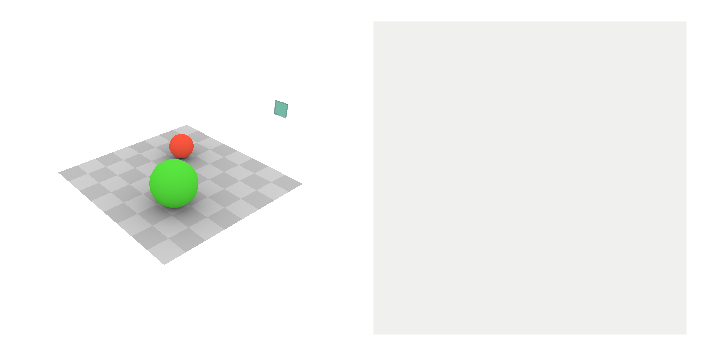
\includegraphics[width=0.65\linewidth]{Figuras/Image_Blanco}
	\caption{Plano de imagen en blanco}
	\label{fig:imageblanco}
\end{figure}

Esto ocurre porque nuestro plano de imagen está expuesto a el ambiente entero, la luz que irradia de cada punto de la escena intersecta con todos los puntos en el plano de imagen.

\begin{figure}[H]
	\centering
	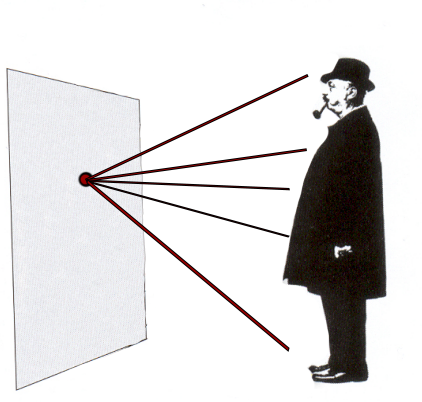
\includegraphics[width=0.5\linewidth]{Figuras/Sensor_Blanco}
	\caption{Un punto del sensor recibe luz de todo el ambiente}
	\label{fig:sensorblanco}
\end{figure}

Se puede solucionar si un punto en el plano de imagen recibe luz de un punto en la escena. Se puede obtener esto si se introduce un objeto que obstruye la luz en todas partes excepto en un punto pequeño.

\begin{figure}[H]
	\centering
	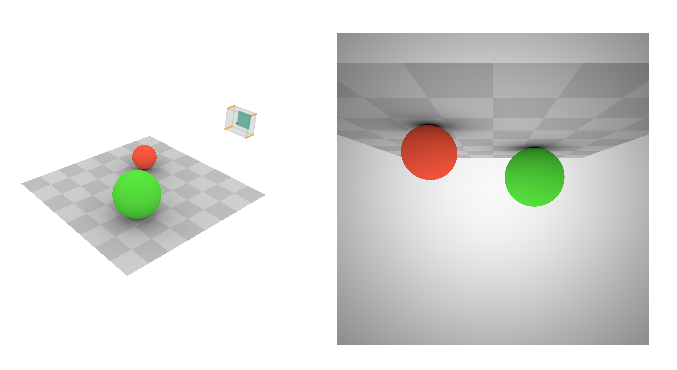
\includegraphics[width=0.65\linewidth]{Figuras/Pinhole}
	\caption{Cámara obscura}
	\label{fig:pinhole}
\end{figure}

\begin{figure}[H]
	\centering
	\includegraphics[width=0.65\linewidth]{Figuras/Pinhole_Pequeño}
	\caption{Cámara obscura con una apertura pequeña}
	\label{fig:pinholepequeno}
\end{figure}

\begin{figure}[H]
	\centering
	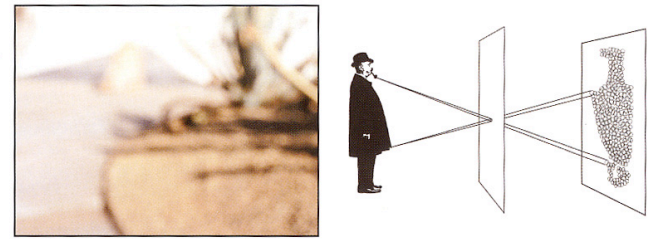
\includegraphics[width=0.65\linewidth]{Figuras/Pinhole_Grande}
	\caption{Cámara obscura con una apertura grande}
	\label{fig:pinholegrande}
\end{figure}

El problema con este método es que, debido a que la apertura es pequeña, la cantidad de luz que entra al plano de imagen es poca.

\pagebreak

\section{Frecuencias Electromagnéticas}
	
	La luz visible forma parte del espectro electromagnético.
	
	\begin{figure}[H]
		\centering
		\includegraphics[width=0.85\linewidth]{Figuras/Espectro_Electromagnético}
		\caption{Espectro electromagnético}
		\label{fig:espectroelectromagnetico}
	\end{figure}

\begin{figure}[H]
	\centering
	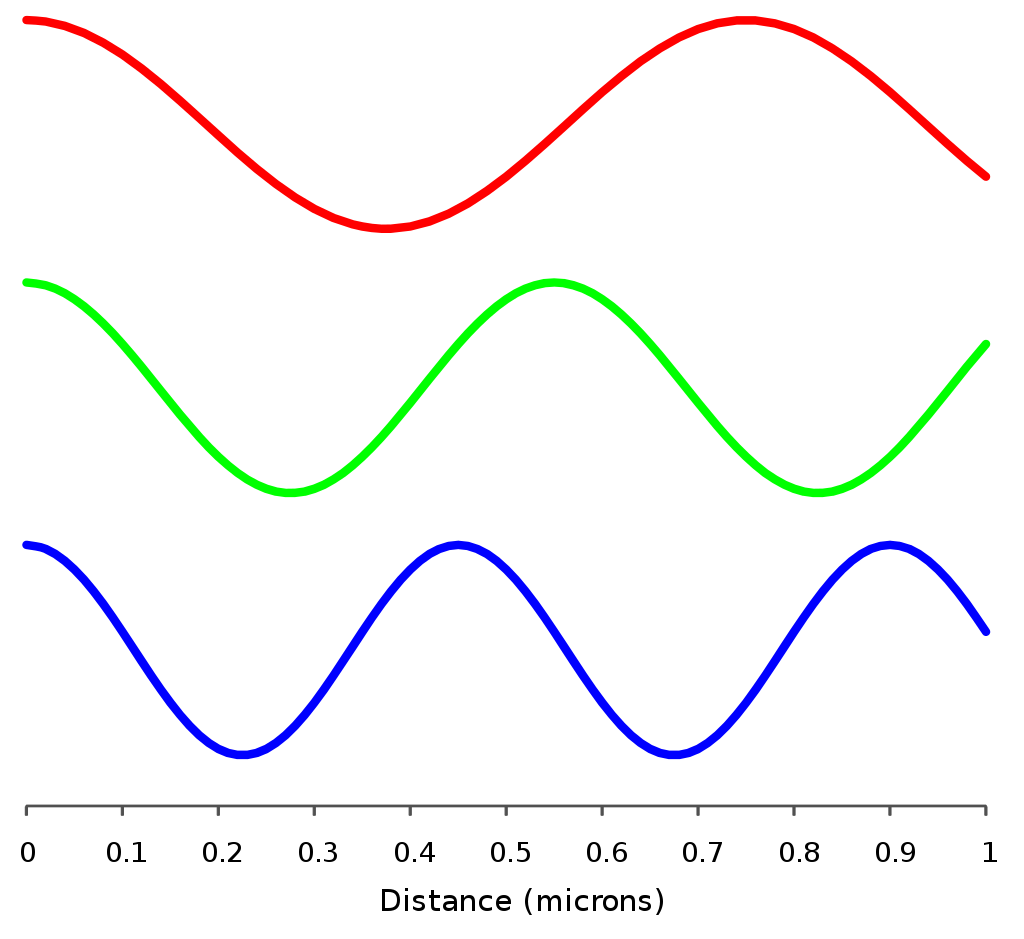
\includegraphics[width=0.45\linewidth]{Figuras/Longitud_de_onda_colores}
	\caption{Lóngitud de onda de los colores primarios}
	\label{fig:longituddeondacolores}
\end{figure}


La radiación electromagnética está compuesta de oscilaciones del campo eléctrico \textbf{E} y el campo magnético \textbf{B}. Estas dos son perpendiculares entre sí y son mutuamente perpendiculares a la dirección de propagación.

\begin{figure}[H]
	\centering
	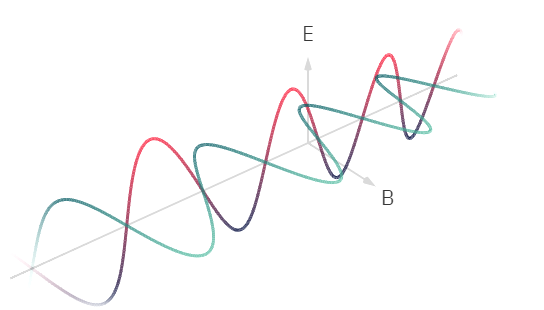
\includegraphics[width=0.55\linewidth]{Figuras/EM_Wave}
	\caption{Onda electromagnética}
	\label{fig:emwave}
\end{figure}

Cuando la luz cambia de material cambia su longitud de onda, esto se relaciona a un cambio de su velocidad de fase $v_p$. Sin embargo, la continuidad de la onda es preservada en todos sus puntos.

\begin{figure}[H]
	\centering
	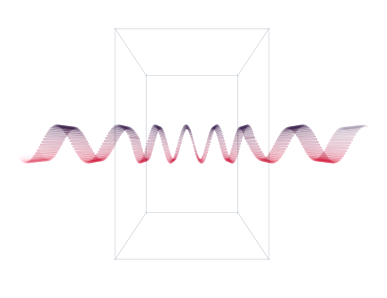
\includegraphics[width=0.55\linewidth]{Figuras/EM_Wave_Vp}
	\caption{Velocidad de fase a través de un medio más denso}
	\label{fig:emwavevp}
\end{figure}

El cambio de velocidad de fase puede ser cuantificado utilizando el \textit{indice de refracción} \textbf{n}.

\begin{align*}
	n=\frac{c}{v_p}
\end{align*}

Mientras más alto el índice de refracción la luz se propaga más lentamente. Aquí hay varios valores del indice de refracción para diferentes materiales:

\begin{center}
\begin{tabular}{c c}
	Vacío & 1.00 \\
	\hline
	Aire & 1.0003 \\
	\hline
	Agua & 1.33 \\
	\hline
	Vidrio & 1.53 \\
	\hline
	Diamante & 2.43 \\
\end{tabular}
\end{center} 

Cuando la dirección de la onda incidente cambia se produce la siguiente onda:

\begin{figure}[H]
	\centering
	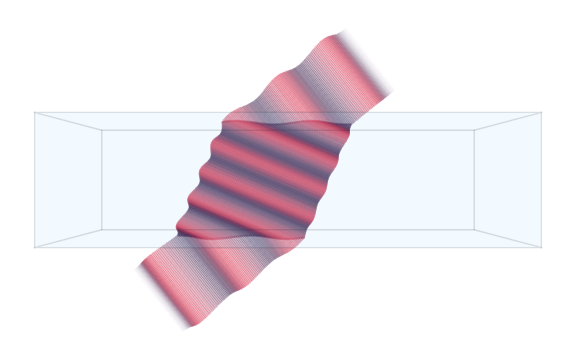
\includegraphics[width=0.60\linewidth]{Figuras/Index_of_refraction}
	\caption{La onda cambia de dirección para preservar su continuidad}
	\label{fig:indexofrefraction}
\end{figure}

La onda en el vidrio tiene una longitud de onda más corta, pero debe mantenerse continua a través de todos sus puntos, por lo tanto la dirección de propagación debe cambiar.	
	
\subsection{Reflexión}

La ley de la reflexión dice que el ángulo de un rayo incidente con la normal $\theta_i$ y el ángulo del rayo de reflexión con la normal $\theta_r$ son iguales
\begin{align*}
	\theta_i = \theta_r
\end{align*}
\begin{figure}[H]
	\centering
	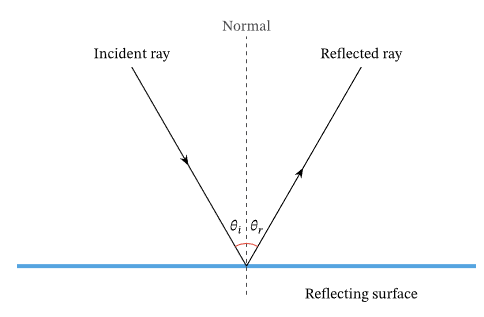
\includegraphics[width=0.65\linewidth]{Figuras/Reflection}
	\caption{Ley de la reflexión}
	\label{fig:reflection}
\end{figure}

\pagebreak

\subsubsection{Reflexión Total Interna}

Existe un ángulo crítico, que depende del indice de refracción de los materiales, en el cual no existe la refracción y solo ocurre reflexión. A esto se le llama reflexión total interna.

\begin{figure}[H]
	\centering
	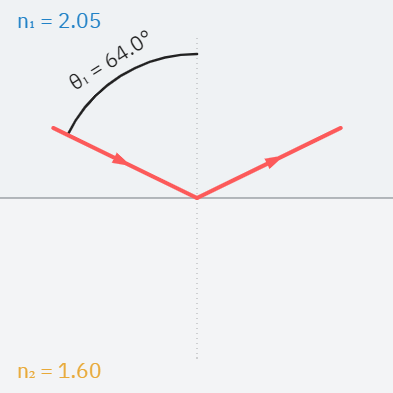
\includegraphics[width=0.50\linewidth]{Figuras/Total_Internal_Reflection}
	\caption{Reflexión total interna}
	\label{fig:totalinternalreflection}
\end{figure}

Es la base del funcionamiento de los cables de fibra óptica, la razón por la que los diamantes brillan es que el corte que tienen provoca que el ángulo crítico por el cual la luz puede escapar por los lados sea muy pequeño y la mayoría de la luz escape por la entrada.

\begin{figure}[H]
	\centering
	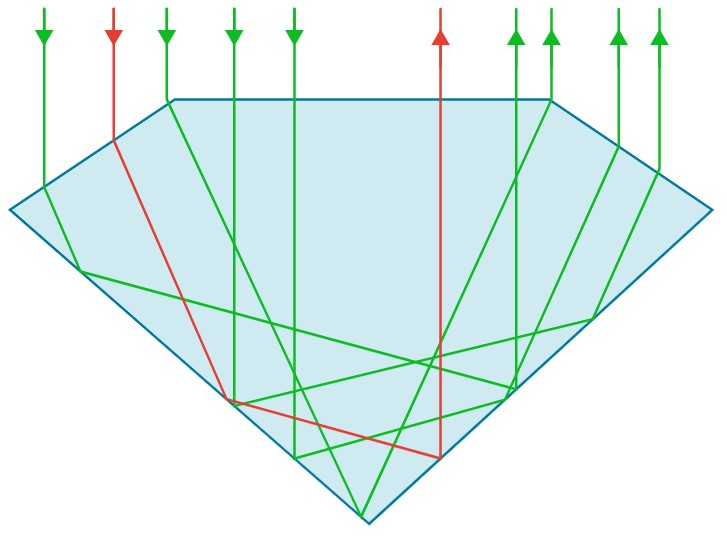
\includegraphics[width=0.45\linewidth]{Figuras/Diamond}
	\caption{Diagrama de la reflexión total interna en un diamante}
	\label{fig:diamond}
\end{figure}

\pagebreak

También es la explicación de la ventana de Snell que ocurre bajo el agua.

\begin{figure}[H]
	\centering
	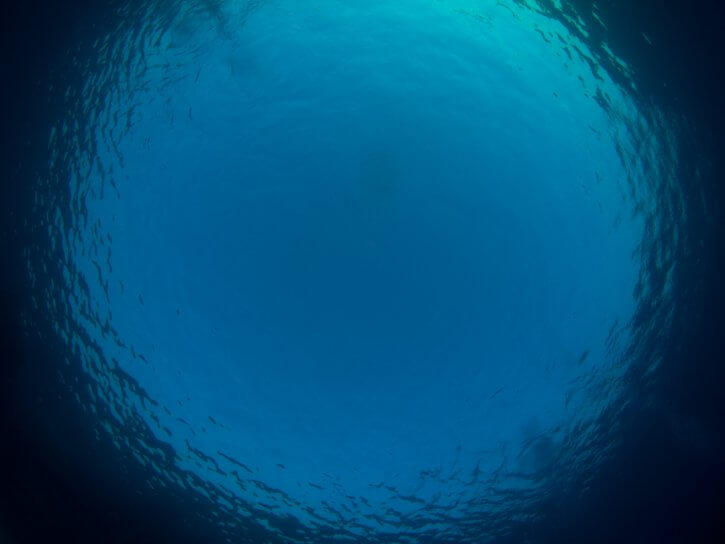
\includegraphics[width=0.6\linewidth]{Figuras/Snell's_Window_2}
	\caption{Ventana de Snell}
	\label{fig:snellswindow2}
\end{figure}

\begin{figure}[H]
	\centering
	\includegraphics[width=0.6\linewidth]{Figuras/"Snell's Window"}
	\caption{Diagrama de los rayos de luz en la ventana de Snell}
	\label{fig:snells-window}
\end{figure}



\subsubsection{Imagenes Virtuales en la Reflexión}

Una imagen virtual es la extensión de rayos de tal manera que convergen en otro punto. En reflejos se puede extender los rayos convergentes de esta manera explicando como funciona un espejo.

\begin{figure}[H]
	\centering
	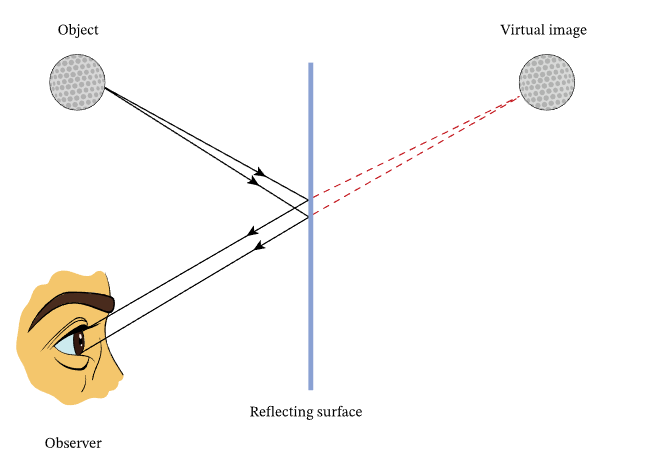
\includegraphics[width=0.65\linewidth]{Figuras/Mirror}
	\caption{Funcionamiento de un espejo}
	\label{fig:mirror}
\end{figure}

También puede explicar los espejismos que se provocan por la diferencia del indice de refracción del aire a diferentes temperaturas.

\begin{figure}[H]
	\centering
	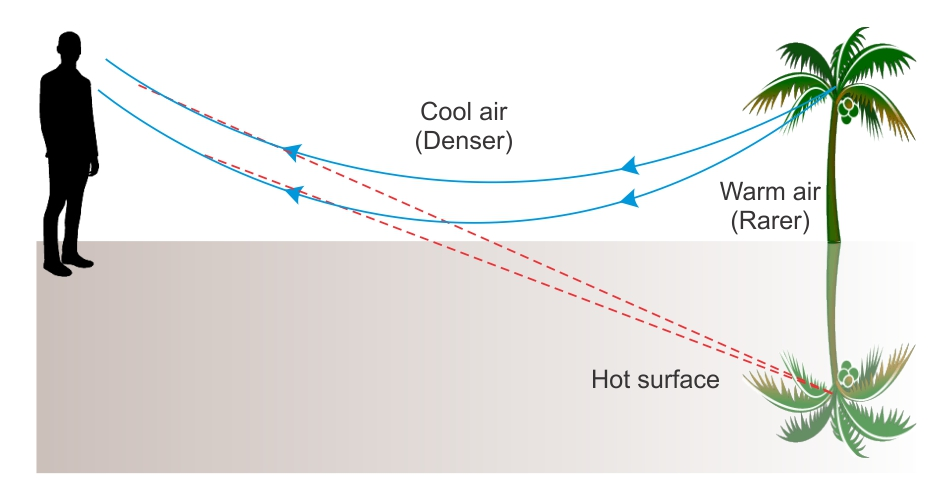
\includegraphics[width=0.75\linewidth]{Figuras/Mirage}
	\caption{Diagrama de un espejismo}
	\label{fig:mirage}
\end{figure}



\subsection{Refracción}

La ley de Snell relaciona el ángulo de incidencia $\theta_1$, el ángulo de refracción $\theta_2$ y los indices de refracción de los diferentes medios:

\begin{align*}
	n_1\sin(\theta_1) = n_2\sin(\theta_2)
\end{align*}

Cuando la luz viaja de un material de menor refracción a uno mayor los rayos de luz cambian su dirección hacia la normal.

\begin{figure}[H]
	\centering
	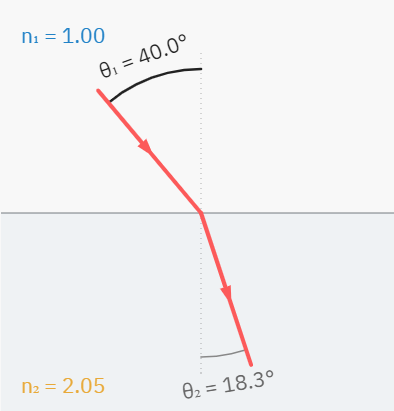
\includegraphics[width=0.5\linewidth]{Figuras/Less_More_Refraction}
	\caption{Los rayos de luz giran hacia la normal cuando van de menor a mayor indice de refracción}
	\label{fig:lessmorerefraction}
\end{figure}

Mientras que cuando viaja de un material con mayor refracción a uno con menor refracción cambian de dirección alejándose de la normal.

\begin{figure}[H]
	\centering
	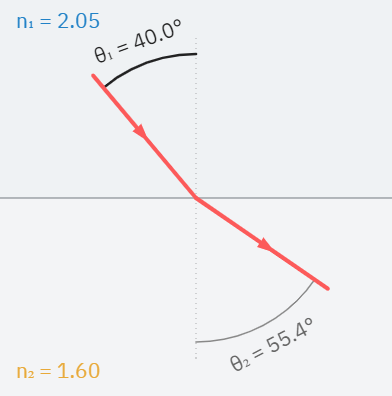
\includegraphics[width=0.5\linewidth]{Figuras/More_Less_Refraction}
	\caption{Los rayos de luz giran alejandose de la normal cuando van de mayor a menor indice de refracción}
	\label{fig:morelessrefraction}
\end{figure}


\subsection{Polarización}

La polarización de una onda electromagnética por convención es designada por la dirección del vector de su campo eléctrico.

La luz u otras radiaciones electromagnéticas de muchas fuentes, como el sol, llamas y luces incandescentes consiste en trenes de onda corta con una mezcla igual de polarizaciones; a esto se le llama luz no polarizada. La luz puede ser polarizada al ser pasada as través de un polarizador.

\begin{figure}[H]
	\centering
	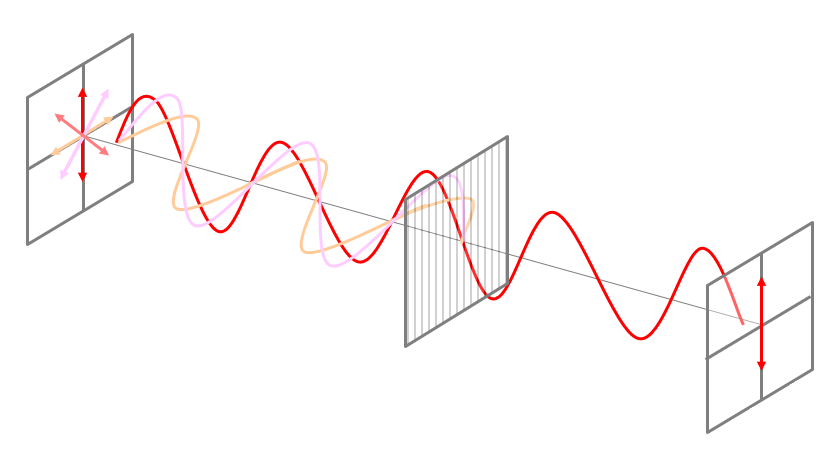
\includegraphics[width=0.65\linewidth]{Figuras/Polarizador}
	\caption{Luz no polarizada pasa por un filtro de polarizado}
	\label{fig:polarizador}
\end{figure}

Si la reflexión y la refracción son perpendiculares provoca que el rayo refractado esté parcialmente polarizado y el rayo reflejado sea totalmente polarizado.


\begin{figure}[H]
	\centering
	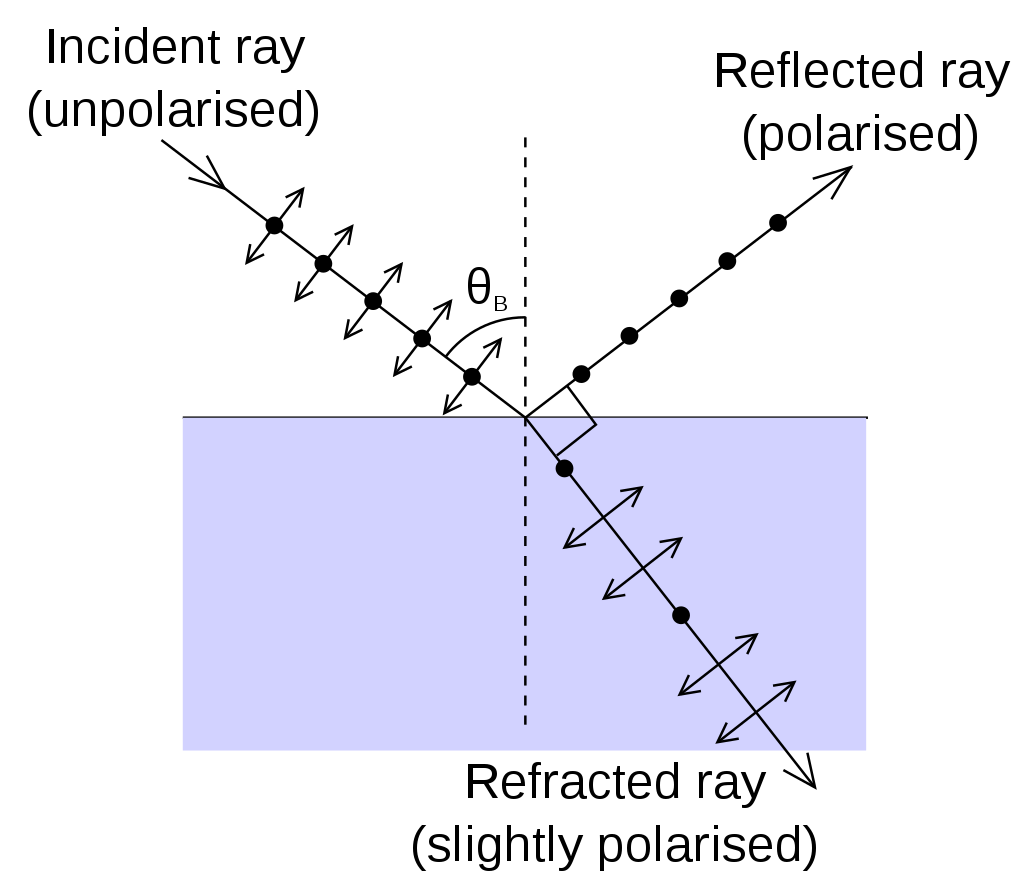
\includegraphics[width=0.60\linewidth]{Figuras/Brewsters_Angle}
	\caption{Diagrama del ángulo de Brewster}
	\label{fig:brewstersangle}
\end{figure}


Si la luz está polarizada se puede eliminar por medio de un filtro polarizado.

\begin{figure}[H]
	\centering
	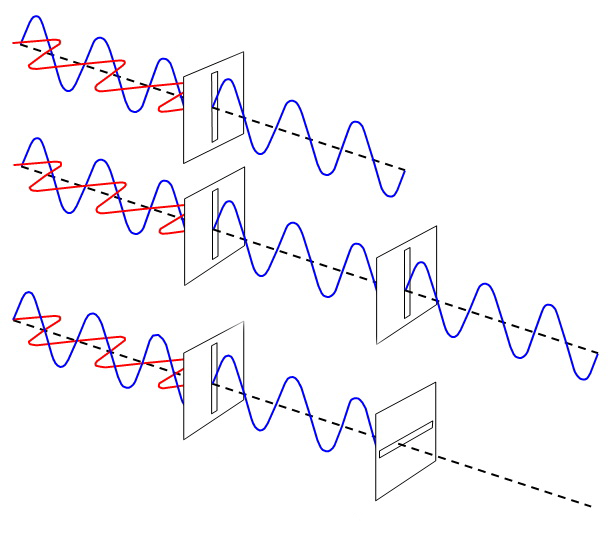
\includegraphics[width=0.75\linewidth]{Figuras/Polarizador_2}
	\caption{En este diagrama la luz es polarizada por el primer filtro y completamente obstruida por el segundo filtro perpendicular al primero}
	\label{fig:polarizador2}
\end{figure}

\begin{figure}[H]
	\centering
	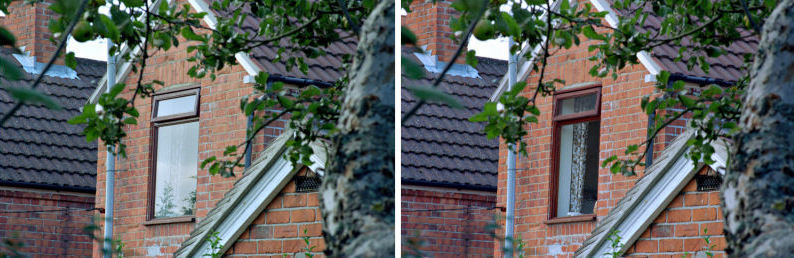
\includegraphics[width=0.85\linewidth]{Figuras/Brewsters_Window}
	\caption{Reflexión eliminada de una ventana con un filtro de polarizado}
	\label{fig:brewsterswindow}
\end{figure}


\section{Lentes}

Utilizando el conocimiento de la refracción podemos ver qué ocurre cuando se modifica el ángulo relativo de una superficie de vidrio.

\begin{figure}[H]
	\centering
	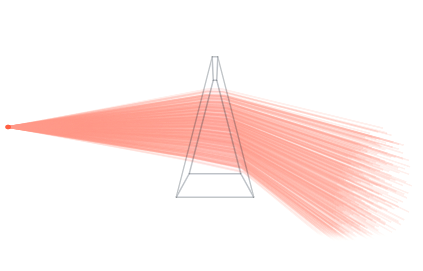
\includegraphics[width=0.65\linewidth]{Figuras/Lens_1}
	\caption{Vidrio con un ángulo en la parte superior}
	\label{fig:lens1}
\end{figure}

\begin{figure}[H]
	\centering
	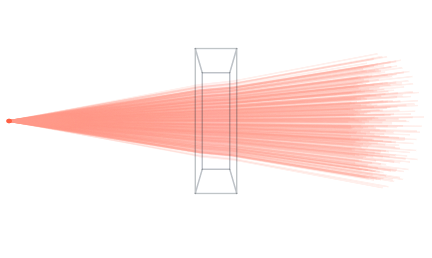
\includegraphics[width=0.65\linewidth]{Figuras/Lens_2}
	\caption{Vidrio recto}
	\label{fig:lens2}
\end{figure}

\begin{figure}[H]
	\centering
	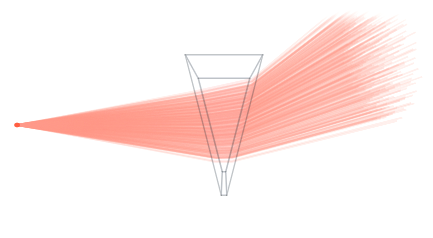
\includegraphics[width=0.65\linewidth]{Figuras/Lens_3}
	\caption{Vidrio con un ángulo en la parte inferior}
	\label{fig:lens3}
\end{figure}

A partir de esto podemos construir un lente que converja todos los rayos de luz en un solo punto.

\begin{figure}[H]
	\centering
	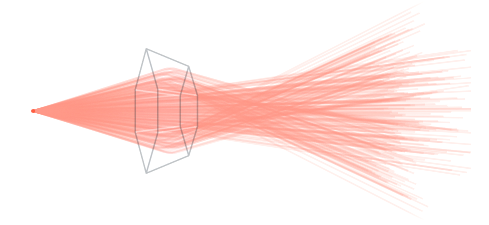
\includegraphics[width=0.65\linewidth]{Figuras/Lens_3_Segments}
	\caption{Lente hecho con los tres segmentos anteriores}
	\label{fig:lens3segments}
\end{figure}

\begin{figure}[H]
	\centering
	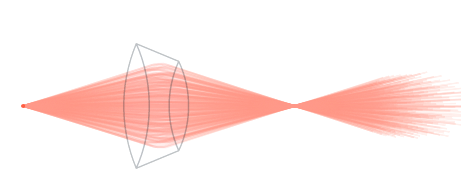
\includegraphics[width=0.65\linewidth]{Figuras/Lens_Infinity_Segments}
	\caption{Lente con una cantidad infinita de segmentos}
	\label{fig:lensinfinitysegments}
\end{figure}

Si este lente es rotacionalmente simétrico creamos un lente delgado. En un lente delgado la distancia entre las superficies de lente $d$ es mucho menor que los radios de curvatura $R_1$ y $R_2$.

\begin{figure}[H]
	\centering
	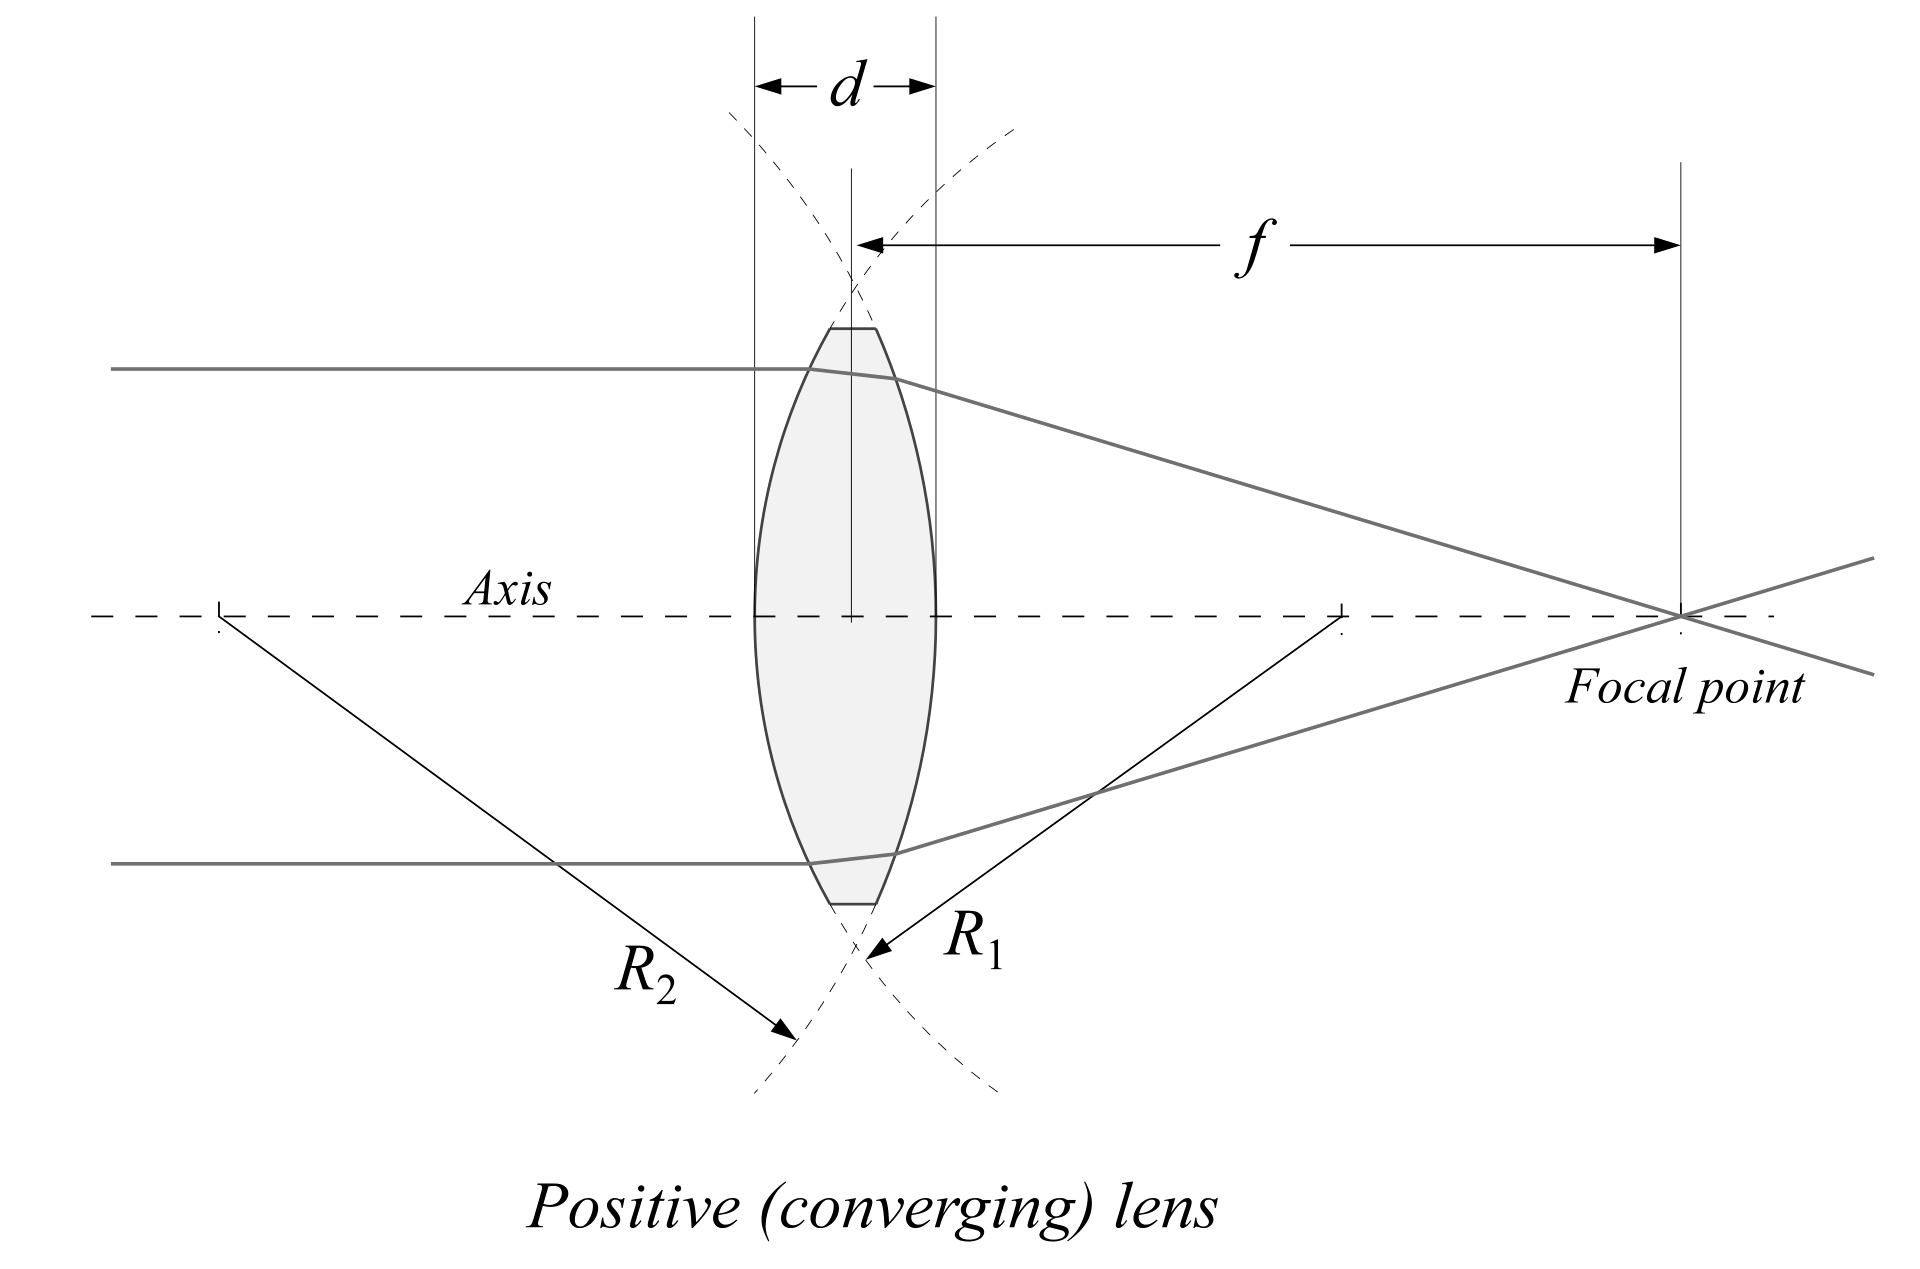
\includegraphics[width=0.75\linewidth]{Figuras/Thin_Lens}
	\caption{Diagrama de un lente delgado}
	\label{fig:thinlens}
\end{figure}


\subsection{Longitud Focal}

La distancia de un \textbf{o}bjeto al lente se le denomina $S_o$, mientras que la distancia del lente al plano de \textbf{i}magen se denomina $S_i$

\begin{figure}[H]
	\centering
	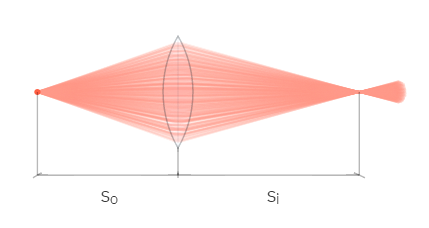
\includegraphics[width=0.65\linewidth]{Figuras/So_Si_Equal}
	\caption{Distancia al objeto y a la imagen}
	\label{fig:sosiequal}
\end{figure}

Si el objeto se encuentra a una distancia infinitamente larga los rayos incidentes al lente son paralelos. La distancia a la cual se convergen rayos paralelos se le denomina longitud focal $f$.

\begin{figure}[H]
	\centering
	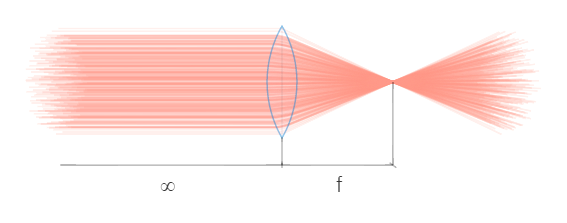
\includegraphics[width=0.65\linewidth]{Figuras/Variables_Longitud_Focal}
	\caption{Los rayos paralelos convergen a la longitud focal}
	\label{fig:variableslongitudfocal}
\end{figure}


Si el lente es delgado se puede obtener con la relación del lente delgado

\begin{align*}
	\frac{1}{f} = \frac{1}{S_o} +\frac{1}{S_i}
\end{align*}

La longitud focal de un lente depende del indice de refracción su material y su forma. En una cámara los vidrios de los lentes son rígidos por lo que se requiere un conjunto de lentes para poder variar la longitud focal.

\begin{figure}[H]
	\centering
	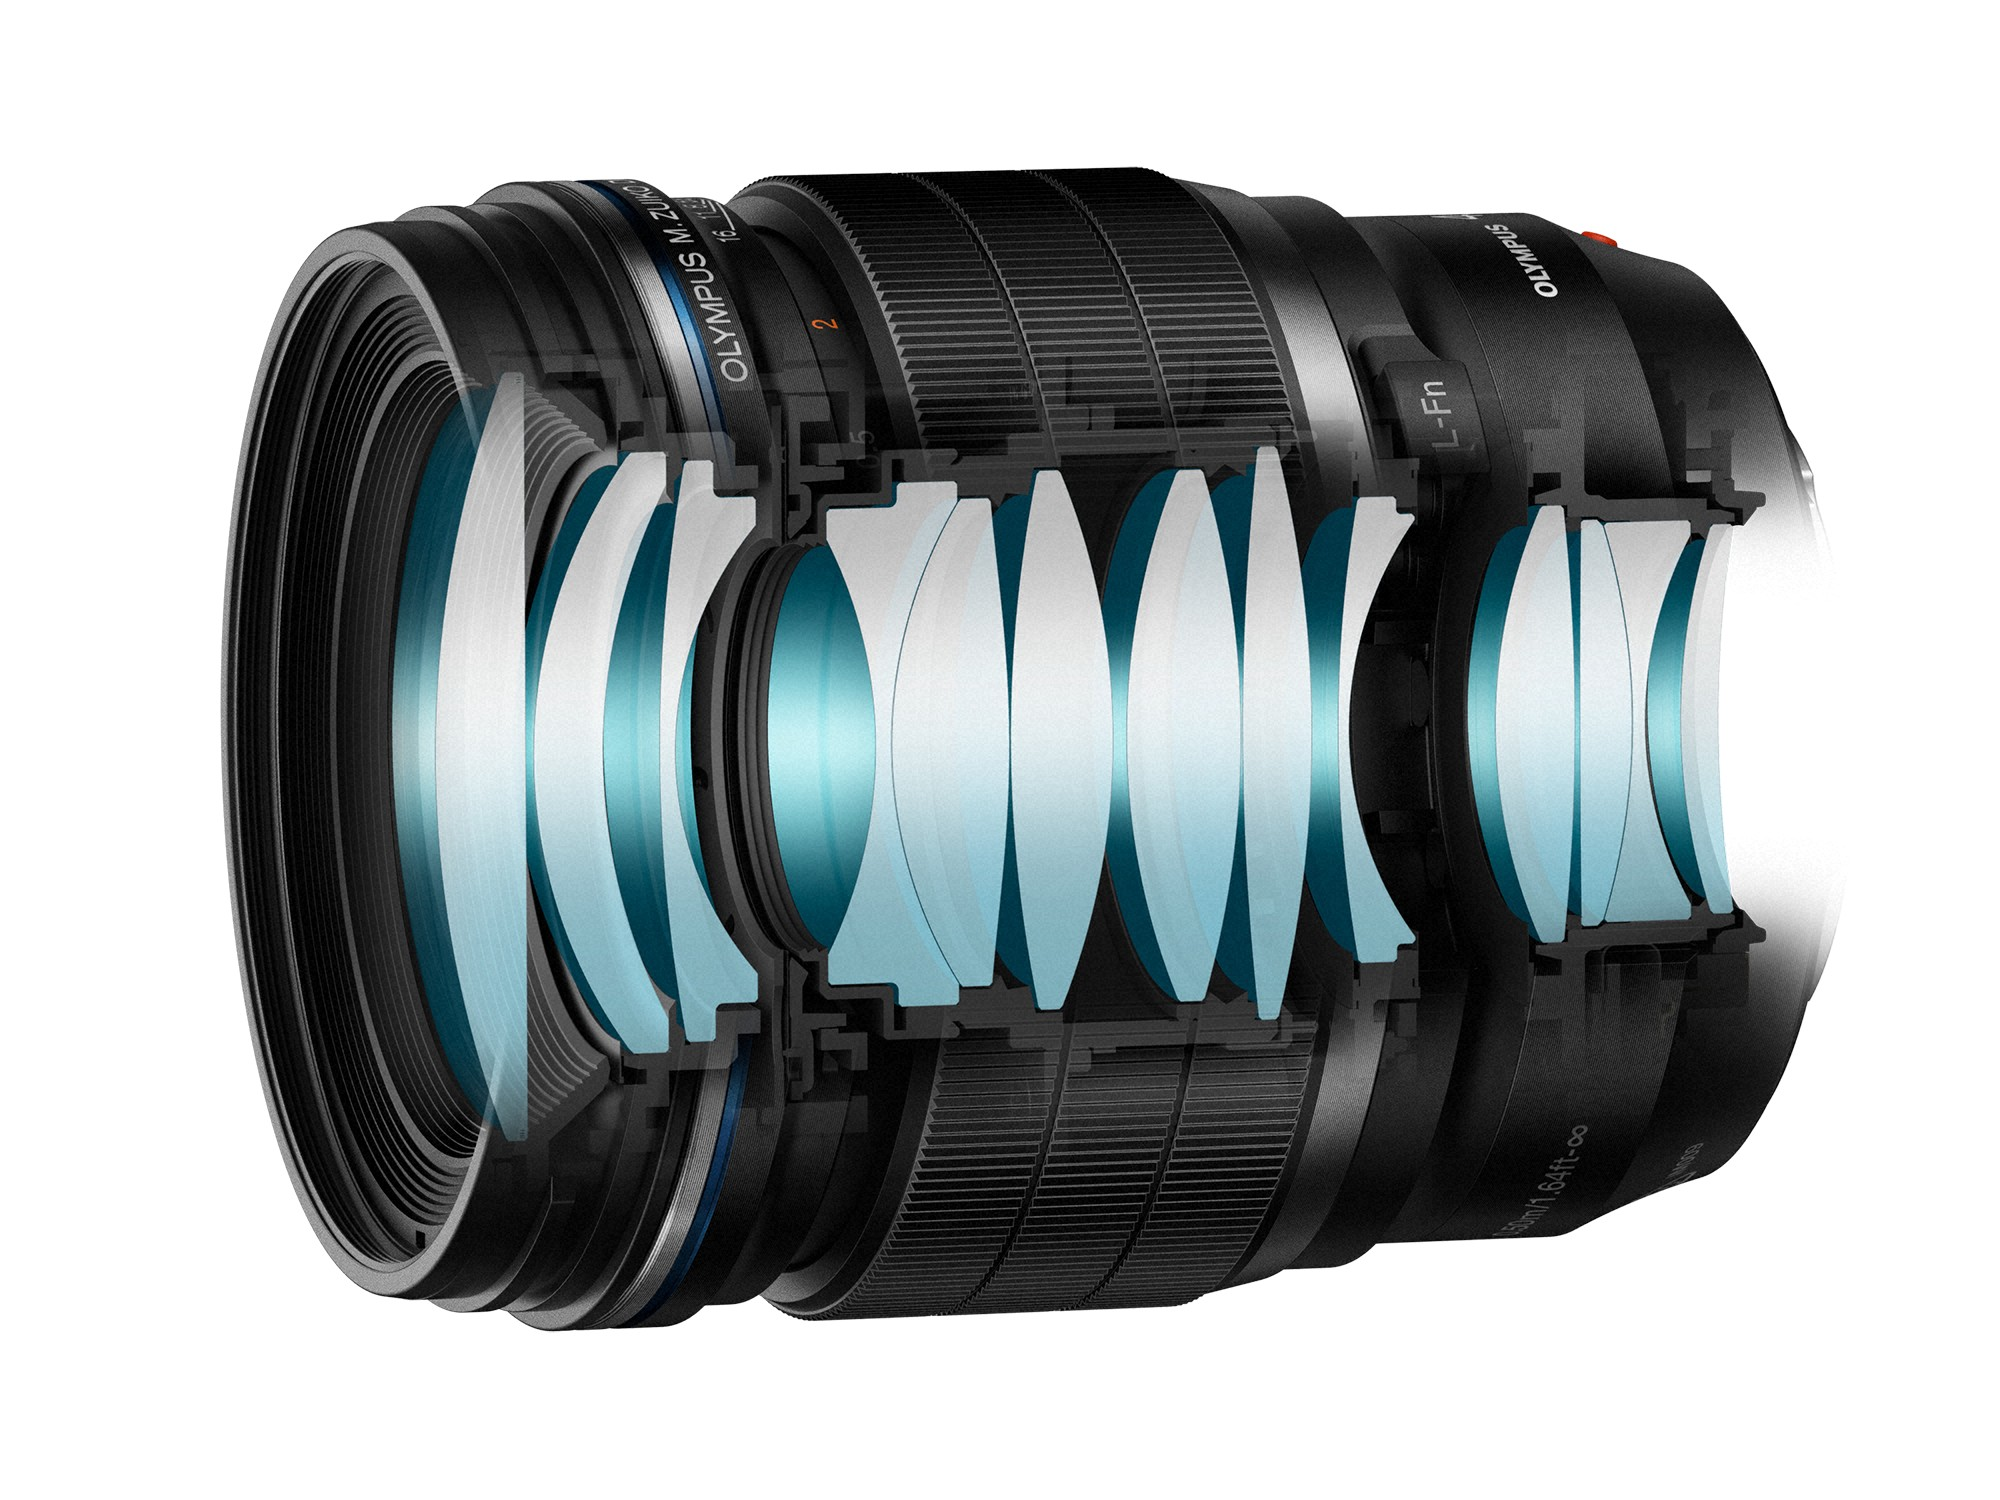
\includegraphics[width=0.60\linewidth]{Figuras/Viariable_focal_length}
	\caption{Un lente de longitud focal variable}
	\label{fig:viariablefocallength}
\end{figure}

Por convención un lente convexo tiene una longitud focal positiva y los rayos de un lente cóncavo pueden ser extendidos hasta encontrar el punto que convergen, este tendría un signo negativo.

\begin{figure}[H]
	\centering
	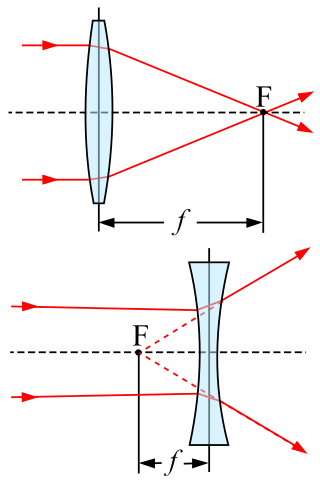
\includegraphics[width=0.50\linewidth]{Figuras/Focal_Length_Concave_Convex}
	\caption{Los lentes concavos tienen una longitud focal positiva y los convexos una longitud negativa}
	\label{fig:focallengthconcaveconvex}
\end{figure}

Debido a que la ecuación de lentes delgados está inversa, frecuentemente es más cómodo trabajar con el inverso de la longitud focal, la dioptría $P$, la cual mide la potencia de un lente. Estos son utilizados por optometristas

\begin{align*}
	P = \frac{1}{f}
\end{align*}

\subsubsection{Crop Factor}

En cámaras digitales, debido a los diferentes tamaños de sensores, cuando se utiliza una longitud focal de la misma magnitud en sensores pequeños se producen imagenes equivalentes a una longitud focal mayor en el sensor grande.

\begin{figure}[H]
	\centering
	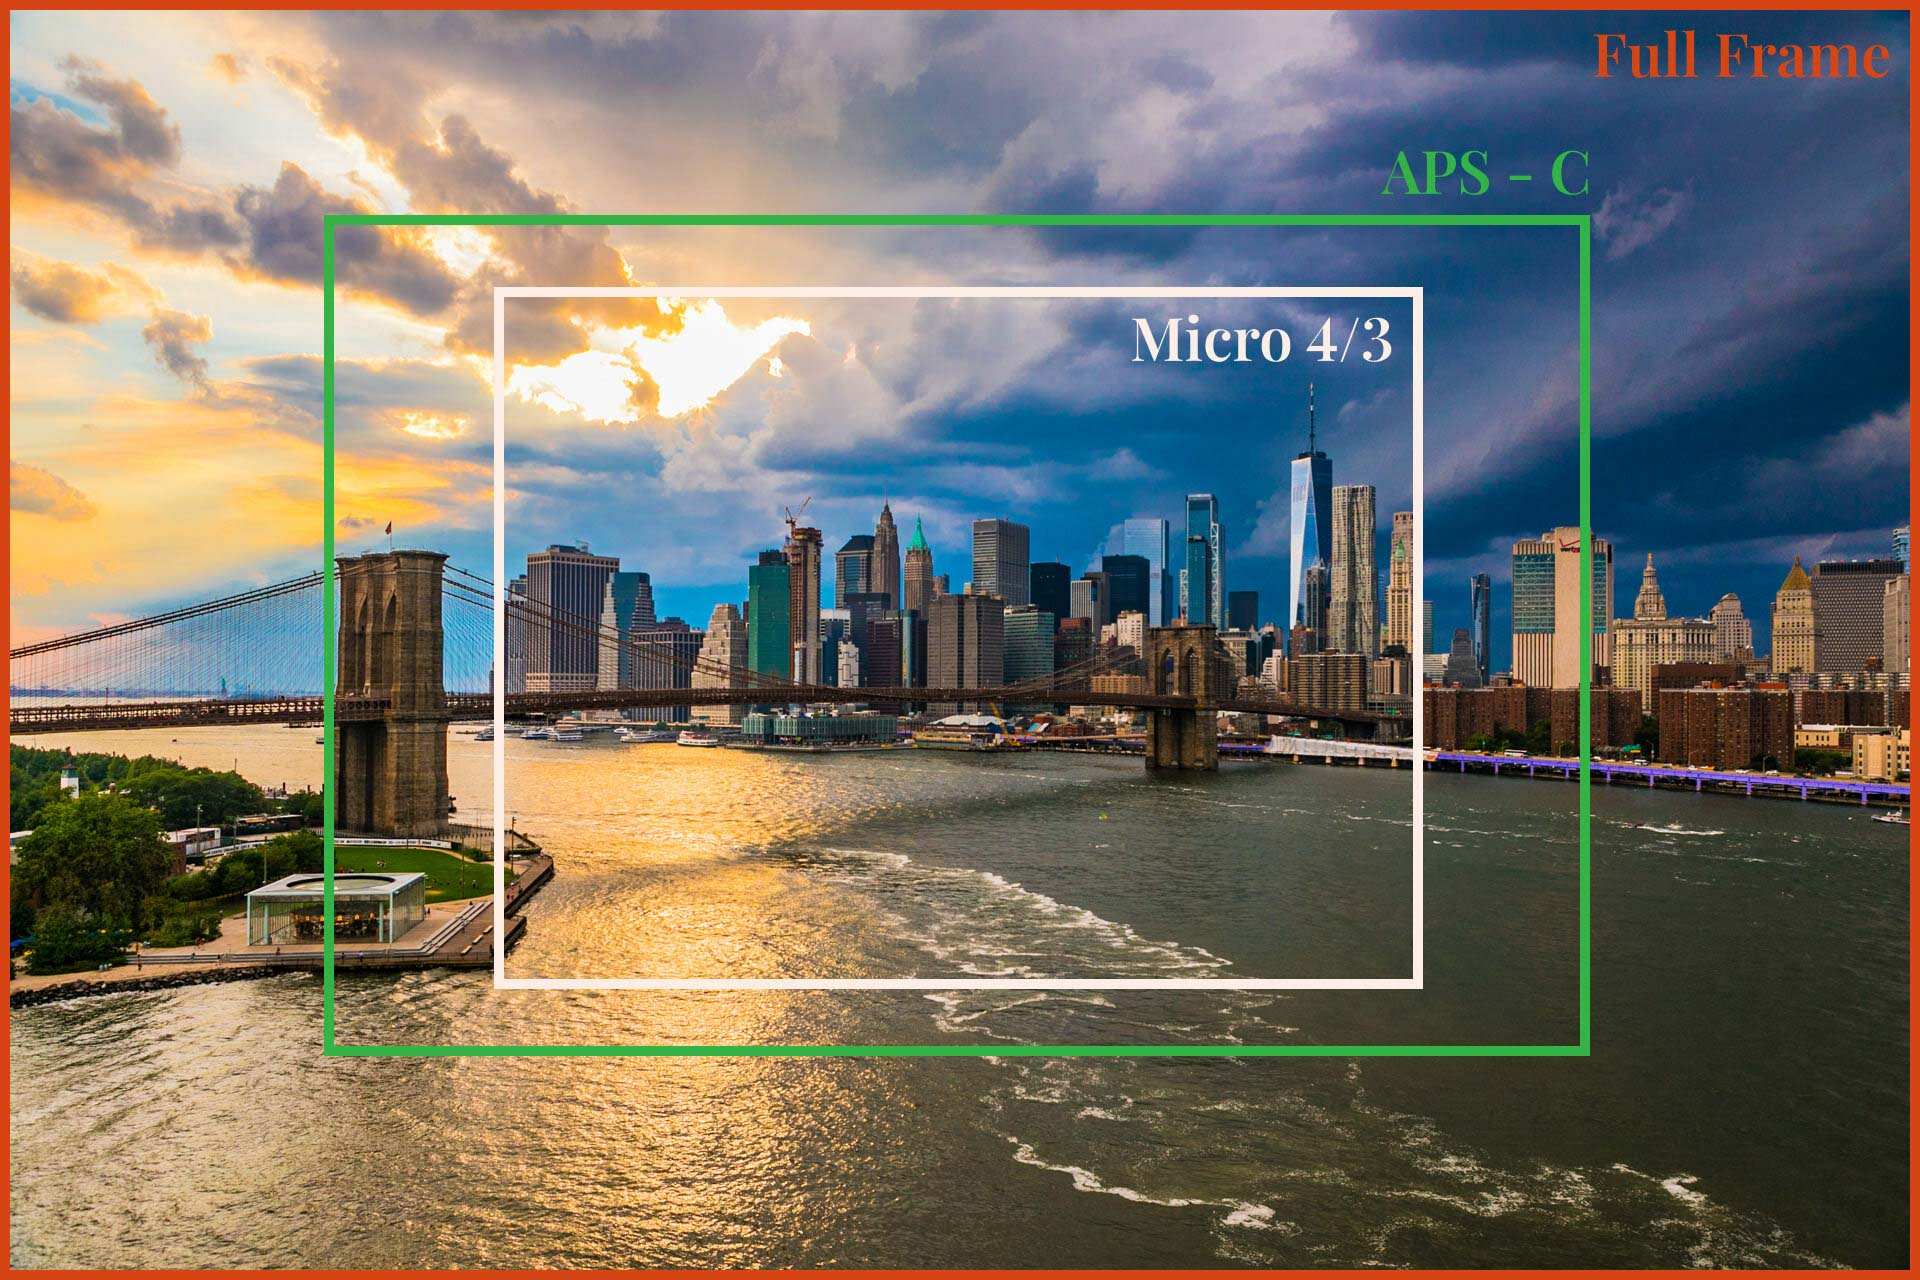
\includegraphics[width=0.70\linewidth]{Figuras/Crop_Factor_Crop}
	\caption{Crop creado por los diferentes tamaños del sensor}
	\label{fig:cropfactorcrop}
\end{figure}

Es decir que para producir una imagen del mismo tamaño se tiene que tomar en cuenta el factor de multiplicación de la longitud focal para producir una imagen con la misma divergencia en sus rayos.

\begin{figure}[H]
	\centering
	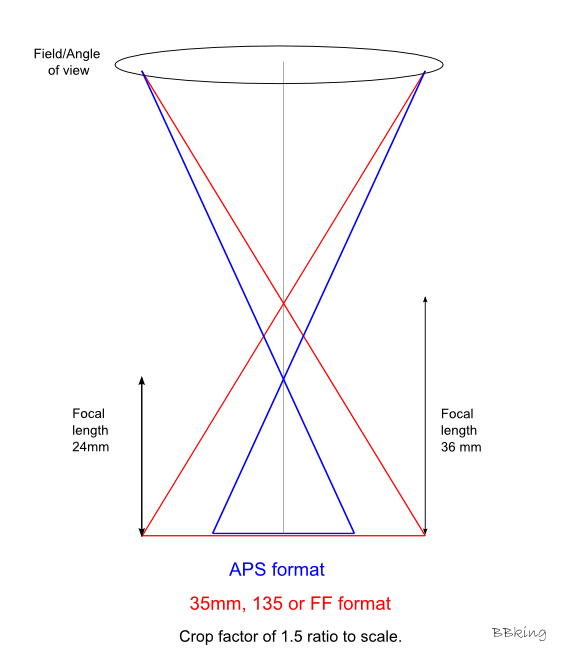
\includegraphics[width=0.60\linewidth]{Figuras/Crop_Factor_Focal_Length}
	\caption{Un lente para sensor APS-C de 24mm es equivalente a un lente para sensor Full Frame de 36mm}
	\label{fig:cropfactorfocallength}
\end{figure}

Se toma como referencia a un sensor Full Frame al cual se la asigna un crop factor de 1. A partir de esto se obtiene el factor de conversión para los demás sensores.

\begin{figure}[H]
	\centering
	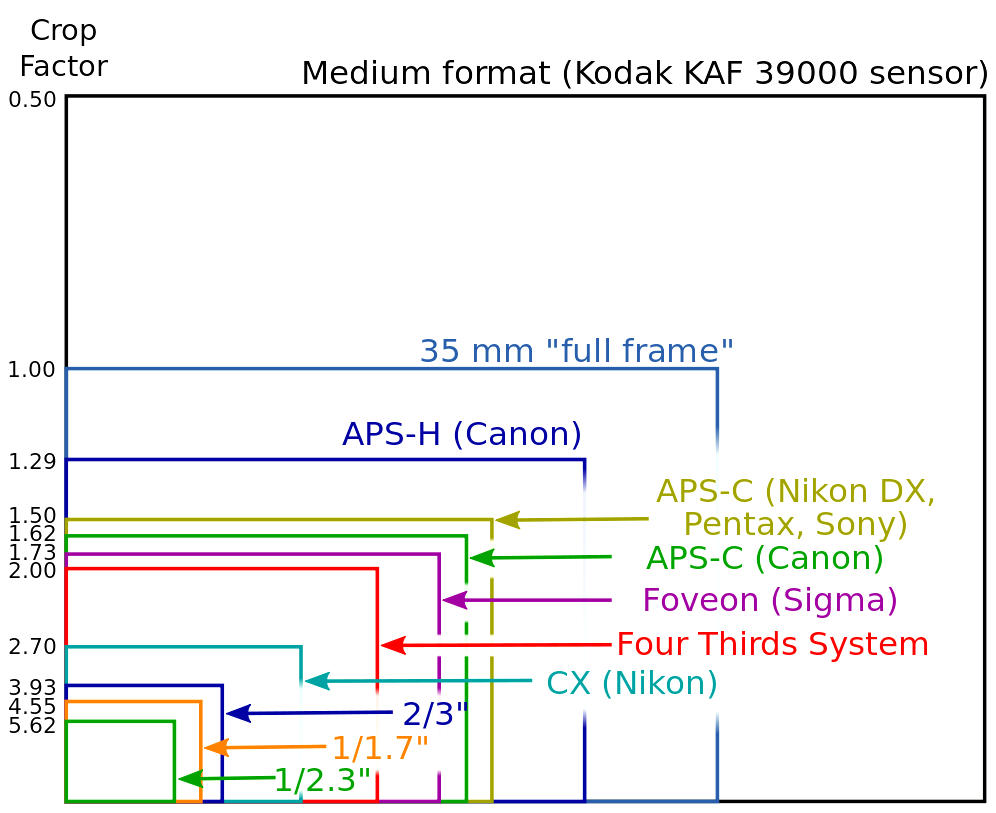
\includegraphics[width=0.65\linewidth]{Figuras/Sensor_Sizes}
	\caption{Tamaños de los diferentes sensores y sus crop factors}
	\label{fig:sensorsizes}
\end{figure}

Por ejemplo, una cámara con un sensor Micro 4/3 y un lente con longitud focal de 25mm es equivalente a un lente con una longitud focal de 50mm para un sensor Full Frame.

\begin{figure}[H]
	\centering
	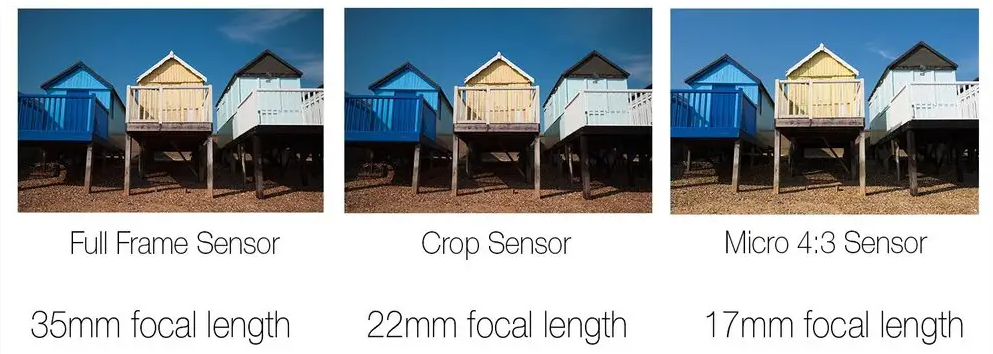
\includegraphics[width=0.75\linewidth]{Figuras/Crop_Factor_Focal_Length_Equivalent}
	\caption{Lentes equivalentes utilizando sensores de diferentes tamaños}
	\label{fig:cropfactorfocallengthequivalent}
\end{figure}


\subsubsection{Imagenes Virtuales en la Refracción}

Si la distancia a la que se encuentra el objeto es igual a la longitud focal los rayos de la distancia de imagen son paralelos.

\begin{figure}[H]
	\centering
	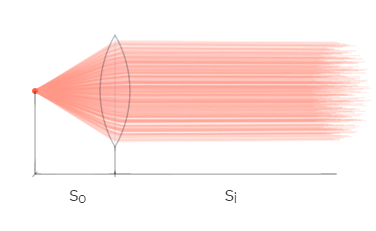
\includegraphics[width=0.65\linewidth]{Figuras/So_Si_Right}
	\caption{Objeto situado a una distancia igual a la longitud focal}
	\label{fig:sosiright}
\end{figure}

En el caso que el objeto se encuentre a una distancia menor que la longitud focal se extienden los rayos de tal manera que crearía una imagen virtual más grande que la imagen real. Este es el principio por el cual funcionan las lupas.

\begin{figure}[H]
	\centering
	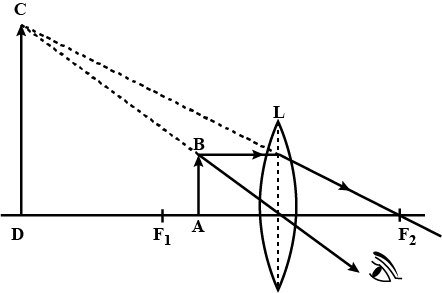
\includegraphics[width=0.65\linewidth]{Figuras/Magnifying_Glass}
	\caption{Un objeto más cerca que la longitud focal produce una imagen virtual de mayor tamaño que el objeto}
	\label{fig:magnifyingglass}
\end{figure}



\subsection{Enfoque}

A diferencia de los lentes en el ojo humano que son capaces de cambiar su forma para enfocar, los lentes de vidrio son rígidos por lo que se debe cambiar la distancia entre el lente y el plano de imagen para poder obtener una imagen enfocada.

\begin{figure}[H]
	\centering
	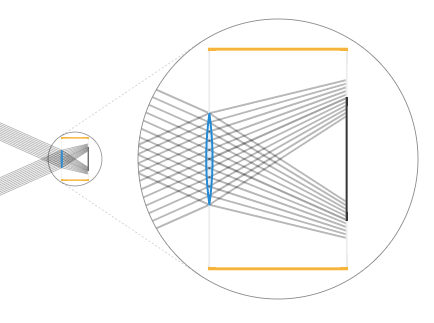
\includegraphics[width=0.45\linewidth]{Figuras/Enfoque_1}
	\caption{Enfoque en frente del objeto}
	\label{fig:enfoque1}
\end{figure}

\begin{figure}[H]
	\centering
	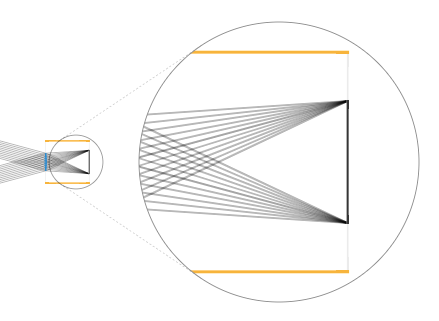
\includegraphics[width=0.45\linewidth]{Figuras/Enfoque_2}
	\caption{Objeto enfocado}
	\label{fig:enfoque2}
\end{figure}

\begin{figure}[H]
	\centering
	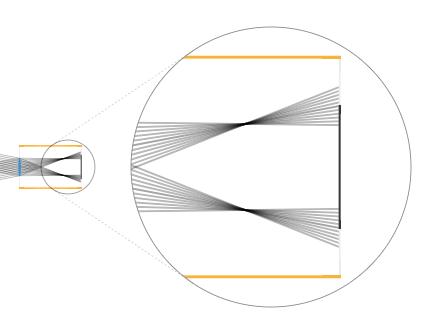
\includegraphics[width=0.45\linewidth]{Figuras/Enfoque_3}
	\caption{Enfoque detrás del objeto}
	\label{fig:enfoque3}
\end{figure}

\subsubsection{Lentes Varifocales y Parafocales}

Los lentes de varifocales, utilizados en cámaras fotográficas, tienen un conjunto de lentes que se encargan de controlar la longitud focal y un grupo también controla el enfoque, por lo que al cambiar la longitud focal también cambia el enfoque.

\begin{figure}[H]
	\centering
	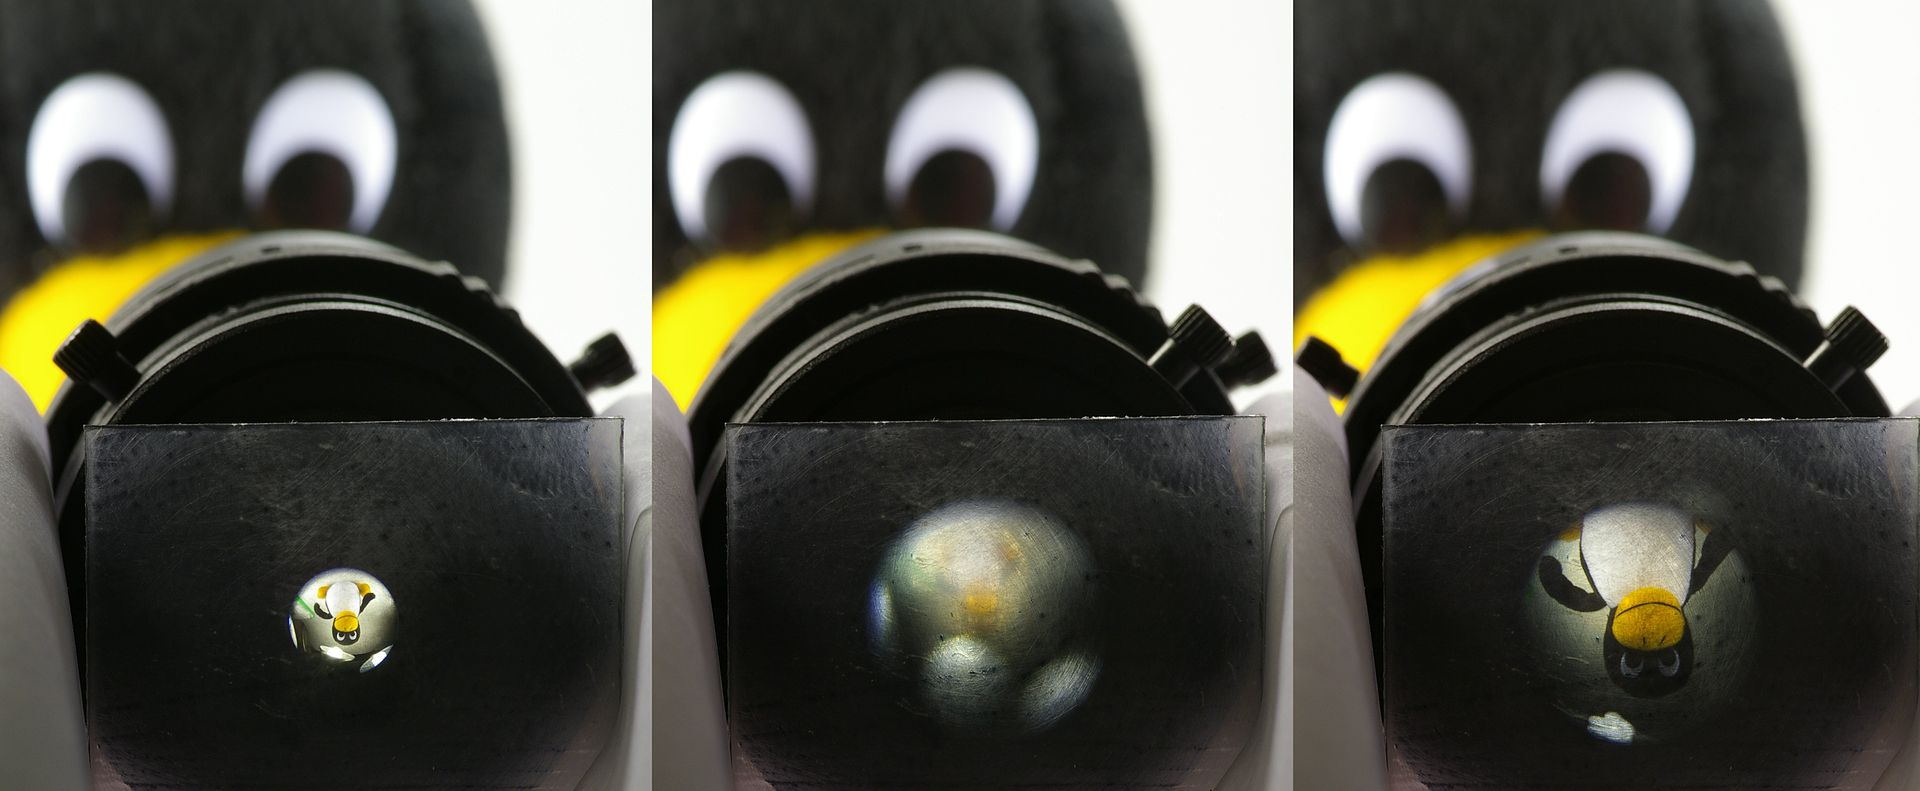
\includegraphics[width=0.75\linewidth]{Figuras/Varifocal_Lens}
	\caption{Un lente varifocal enfocado pierde su enfoque cuando cambia su longitud focal y es necesario reajustarlo}
	\label{fig:varifocallens}
\end{figure}

\begin{figure}[H]
	\centering
	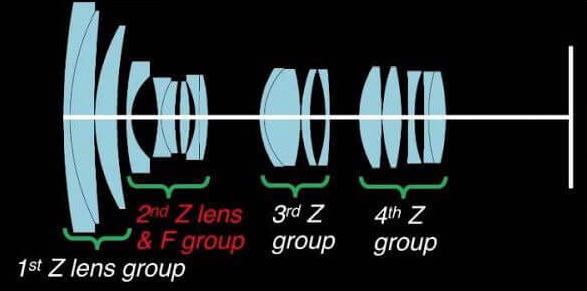
\includegraphics[width=0.75\linewidth]{Figuras/Varifocal_Lens_2.jpg}
	\caption{Un lente varifocal tiene un conjunto de lentes que controlan la longitud focal y el enfoque}
	\label{fig:varifocallens2}
\end{figure}

Un lente parfocal, utilizados en cámaras de video, tiene los lentes de enfoque y longitud focal separados, por lo cual puede mantenerse enfocado mientras cambia la longitud focal.

\begin{figure}[H]
	\centering
	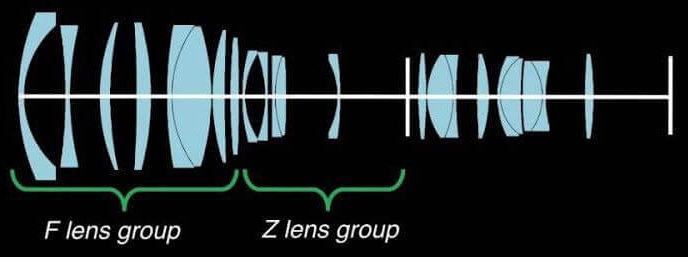
\includegraphics[width=0.75\linewidth]{Figuras/Parfocal_Lens}
	\caption{Un lente parfocal tiene los lentes para la longitud focal y enfoque separados}
	\label{fig:parfocallens}
\end{figure}

\pagebreak

\subsubsection{Enfoque en el ojo humano}

Una persona con miopía tiene el ojo demasiado grande y los rayos de luz convergen antes de la retina, es necesario un lente cóncavo para ajustar el enfoque.

\begin{figure}[H]
	\centering
	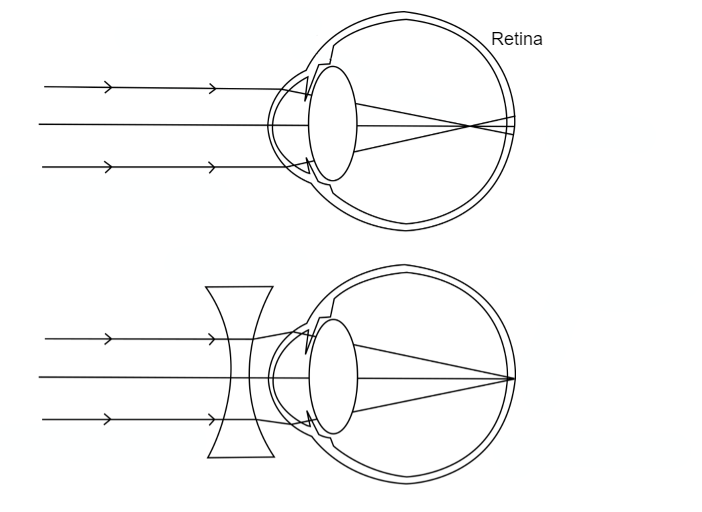
\includegraphics[width=0.6\linewidth]{Figuras/Miopia}
	\caption{Un ojo con miopía requiere de un lente cóncavo}
	\label{fig:miopia}
\end{figure}

Una persona con hipermetropía tiene el ojo demasiado pequeño y los rayos de luz convergen más allá de la retina, es necesario un lente convexo para ajustar el enfoque.

\begin{figure}[H]
	\centering
	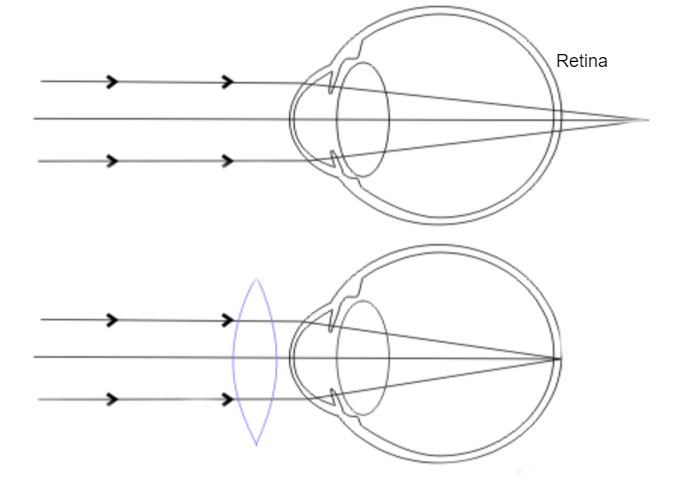
\includegraphics[width=0.6\linewidth]{Figuras/Hipermetropia}
	\caption{Un ojo con hipermetropía requiere de un lente convexo}
	\label{fig:hipermetropia}
\end{figure}


\subsection{Aberraciones}

Las aberraciones son una propiedad de los sistemas ópticos, como lentes, que provocan que la luz sea esparcida sobre una región en el espacio en vez de ser enfocada en un punto. Causan que la imagen sea borrosa o distorsionada.

Las aberraciones monocromáticas ocurren por la geometría del lente y ocurren cuando la luz es reflejada y refractada. Las más comunes son:

\begin{itemize}
	\item Desenfoque
	\item Esférica
	\item Coma
	\item Astigmatismo
	\item Curvatura del campo
	\item Distorsión de imagen
\end{itemize}

El desenfoque tipicamente no se considera una aberración óptica ya que puede ser corregido al mover el lente o la cámara.

Las aberraciones cromáticas ocurren por la dispersión de la luz, la cual es la variación del indice de refracción del lente con la longitud de onda. No ocurren cuando se utiliza luz monocromática.

\begin{itemize}
	\item Axial o Longitudinal
	\item Lateral o Transversa
\end{itemize}


\subsubsection{Esférica}

Un lente perfecto tiene forma de parábola, pero los lentes reales tienen una forma esférica lo cual provoca que no todos los puntos se enfoquen a la misma distancia.

\begin{figure}[H]
	\centering
	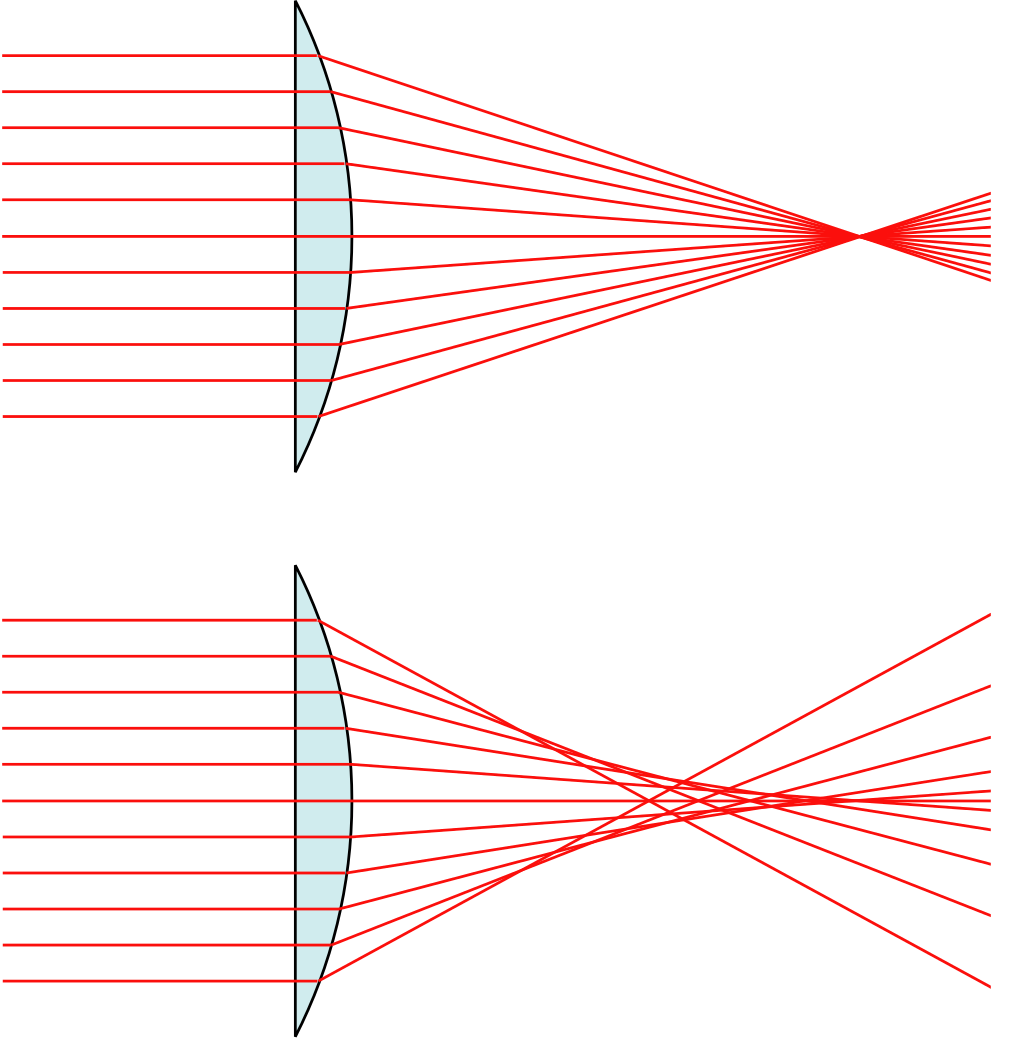
\includegraphics[width=0.55\linewidth]{Figuras/Spherical_Aberration}
	\caption{Un lente esférico produce áreas fuera de enfoque en sus extremos}
	\label{fig:sphericalaberration}
\end{figure}

\begin{figure}[H]
	\centering
	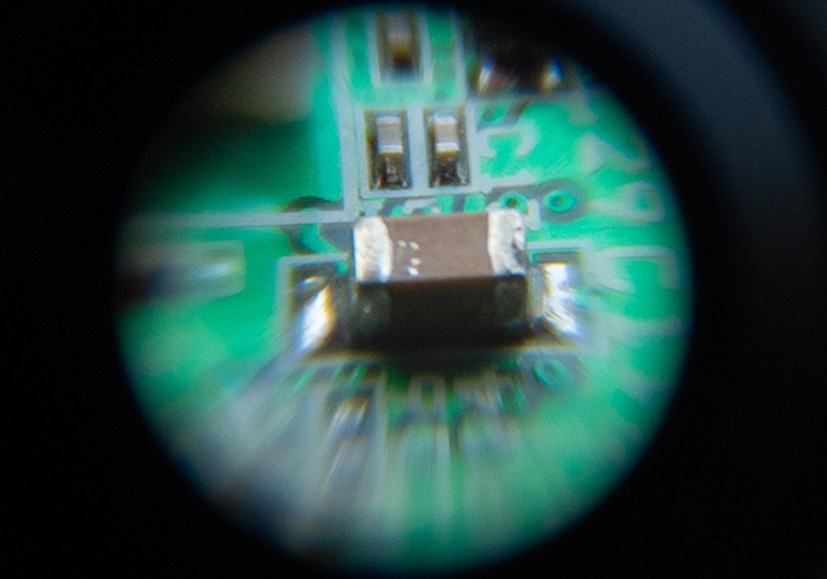
\includegraphics[width=0.65\linewidth]{Figuras/Spherical_Aberration_2}
	\caption{Imagen con aberración esférica severa}
	\label{fig:sphericalaberration2}
\end{figure}


\subsubsection{Coma}

Un objeto fuera de eje produce converge los rayos de luz en diferentes puntos

\begin{figure}[H]
	\centering
	\includegraphics[width=0.65\linewidth]{Figuras/Coma}
	\caption{Un objeto fuera de eje produce enfoques a lo largo de diferentes puntos}
	\label{fig:coma}
\end{figure}

\begin{figure}[H]
	\centering
	\includegraphics[width=0.65\linewidth]{Figuras/Coma_2}
	\caption{Se le llama coma porque la aberración hace que las estrellas parezcan cometas}
	\label{fig:coma2}
\end{figure}

\begin{figure}[H]
	\centering
	\includegraphics[width=0.65\linewidth]{Figuras/Coma_3}
	\caption{Coma en astrofotografía}
	\label{fig:coma3}
\end{figure}

\begin{figure}[H]
	\centering
	\includegraphics[width=0.65\linewidth]{Figuras/Coma_4}
	\caption{Detalles de la imagen anterior}
	\label{fig:coma4}
\end{figure}


\subsubsection{Astigmatismo}

Ocurre cuando los planos perpendiculares de un lente enfocan a una distancia diferente.

\begin{figure}[H]
	\centering
	\includegraphics[width=0.65\linewidth]{Figuras/Astigmatismo}
	\caption{Los dos ejes del lente enfocan a distancias diferentes}
	\label{fig:astigmatismo}
\end{figure}

\begin{figure}[H]
	\centering
	\includegraphics[width=0.85\linewidth]{Figuras/Astigmatismo_2}
	\caption{Efectos del astigmatismo}
	\label{fig:astigmatismo2}
\end{figure}

\begin{figure}[H]
	\centering
	\includegraphics[width=0.65\linewidth]{Figuras/Astigmatismo_3}
	\caption{Astigmatismo en astrofotografía}
	\label{fig:astigmatismo3}
\end{figure}

\begin{figure}[H]
	\centering
	\includegraphics[width=0.65\linewidth]{Figuras/Astigmatismo_4}
	\caption{Detalles de la imagen anterior}
	\label{fig:astigmatismo4}
\end{figure}

\subsubsection{Curvatura del Campo}

A diferencia del ojo humano que tiene un plano de imagen curvo, los planos de imagen típicamente son superficies planas por lo cual crea una distorsión al proyectar la imagen. Esto produce que una imagen esté menos enfocada en sus ejes cuando se enfoca en el centro y viceversa.

\begin{figure}[H]
	\centering
	\includegraphics[width=0.75\linewidth]{Figuras/Field_Curvature}
	\caption{Un lente produce una imagen en un plano curvo, mientras que los sensores comunmente son planos}
	\label{fig:fieldcurvature}
\end{figure}

\begin{figure}[H]
	\centering
	\includegraphics[width=0.85\linewidth]{Figuras/Field_Curvature_2}
	\caption{Curvatura de campo donde el centro está más desenfocado que los ejes}
	\label{fig:fieldcurvature2}
\end{figure}

\subsubsection{Distorsión de Imagen}

Es cualquier desviación de una proyección rectilinea, una proyección en la cual lineas rectas en una escena permanecen rectas en la imagen.

\begin{figure}[H]
	\centering
	\includegraphics[width=0.40\linewidth]{Figuras/Distorsion_1}
	\caption{Diagrama de la distorsión de barril}
	\label{fig:distorsion1}
\end{figure}

\begin{figure}[H]
	\centering
	\includegraphics[width=0.40\linewidth]{Figuras/Distorsion_2}
	\caption{Diagrama de la distorsión de cojín}
	\label{fig:distorsion2}
\end{figure}

\begin{figure}[H]
	\centering
	\includegraphics[width=0.40\linewidth]{Figuras/Distorsion_3}
	\caption{Diagrama de la distorsión de bigote}
	\label{fig:distorsion3}
\end{figure}

\begin{figure}[H]
	\centering
	\includegraphics[width=0.60\linewidth]{Figuras/Distorsion_4}
	\caption{Distorsión de barril en una imagen}
	\label{fig:distorsion4}
\end{figure}

\subsubsection{Axial o Longitudinal}

Las diferentes longitudes de onda que conforman los colores son enfocados a una distancia diferente a lo largo del eje axial

\begin{figure}[H]
	\centering
	\includegraphics[width=0.70\linewidth]{Figuras/Axial_Aberration}
	\caption{Diagrama de aberración cromática axial}
	\label{fig:axialaberration}
\end{figure}

\begin{figure}[H]
	\centering
	\includegraphics[width=0.65\linewidth]{Figuras/Axial_Aberration_2}
	\caption{Aberración cromática axial en una imagen, nótese la franja morada en frente y la franja verde atrás}
	\label{fig:axialaberration2}
\end{figure}

Puede ser solucionado con un doblete acromático.

\begin{figure}[H]
	\centering
	\includegraphics[width=0.70\linewidth]{Figuras/Axial_Aberration_3}
	\caption{Doblete Acromático}
	\label{fig:axialaberration3}
\end{figure}

\subsubsection{Lateral o Transversa}

Las diferentes longitudes de onda se enfocan en puntos diferentes en el plano de imagen.

\begin{figure}[H]
	\centering
	\includegraphics[width=0.65\linewidth]{Figuras/Lateral_Aberration}
	\caption{Las longitudes de onda se enfocan en diferentes puntos en el plano de imagen}
	\label{fig:lateralaberration}
\end{figure}

\begin{figure}[H]
	\centering
	\includegraphics[width=0.65\linewidth]{Figuras/Lateral_Aberration_2}
	\caption{Aberración cromática lateral en una imagen}
	\label{fig:lateralaberration2}
\end{figure}






\subsection{Otras Imperfecciones}

\subsubsection{Viñeteado}

El viñeteado ocurre debido a que los rayos que no son perpendiculares al plano de a apertura no son circulares y son ovalados, lo cual reduce la cantidad de luz que entra conforme incrementa ángulo y produce bordes subexpuestos en la imagen. Esto ocurre comúnmente con cámaras de juguete.

\begin{figure}[H]
	\centering
	\includegraphics[width=0.45\linewidth]{Figuras/Vignetting_lzquierdo}
	\caption{Vista lateral izquierda de la apertura, su proyección es un ovalo}
	\label{fig:vignettinglzquierdo}
\end{figure}

\begin{figure}[H]
	\centering
	\includegraphics[width=0.35\linewidth]{Figuras/Vignetting_Medio}
	\caption{Vista frontal de la apertura, su proyección es un círculo}
	\label{fig:vignettingmedio}
\end{figure}

\begin{figure}[H]
	\centering
	\includegraphics[width=0.35\linewidth]{Figuras/Vignetting_Derecho}
	\caption{Vista lateral derecha de la apertura, su proyección es un ovalo}
	\label{fig:vignettingderecho}
\end{figure}

\begin{figure}[H]
	\centering
	\includegraphics[width=0.55\linewidth]{Figuras/Vignetting_Real}
	\caption{Viñeteado en una imagen a blanco y negro}
	\label{fig:vignettingreal}
\end{figure}

\begin{figure}[H]
	\centering
	\includegraphics[width=0.65\linewidth]{Figuras/Vignetting_Real2}
	\caption{Viñeteado en una imagen a color}
	\label{fig:vignettingreal2}
\end{figure}

\subsubsection{Destello de Lente}

Ocurre cuando la luz es refractada en un sistema de lentes. Puede manifestarse como deslumbramiento, en el cual reduce el contraste y saturación de colores de la imagen, o como artefactos con la forma de la apertura.

\begin{figure}[H]
	\centering
	\includegraphics[width=0.65\linewidth]{Figuras/Flare}
	\caption{Diagrama del destello de lente}
	\label{fig:flare}
\end{figure}

\begin{figure}[H]
	\centering
	\includegraphics[width=0.45\linewidth]{Figuras/Flare_2}
	\caption{Deslumbramiento en una imagen}
	\label{fig:flare2}
\end{figure}

\begin{figure}[H]
	\centering
	\includegraphics[width=0.45\linewidth]{Figuras/Flare_3}
	\caption{Artefactos de destello en una imagen}
	\label{fig:flare3}
\end{figure}

\pagebreak

Los lentes actuales contienen capas delgadas de materiales que eliminan reflejos de una longitud de onda específica. Las cámaras también están pintadas de negro por dentro y tienen formas diseñadas para obstruir el paso de la luz que intenta reflejarse por dentro.

También se le puede agregar una parasol al lente para evitar la entrada de rayos de luz fuera de eje.

\begin{figure}[H]
	\centering
	\includegraphics[width=0.55\linewidth]{Figuras/Lens_Hood}
	\caption{Cámara Sony A7s con parasol en el lente}
	\label{fig:lenshood}
\end{figure}



\section{Exposición}

La exposición de una imagen es controlada por tres factores: la velocidad de obturación, la apertura del diafragma y el ISO. De esos tres se le pone un enfoque a la velocidad y apertura ya que esos dos parámetros controlan la cantidad de luz que entra al plano de imagen.

\begin{figure}[H]
	\centering
	\includegraphics[width=0.65\linewidth]{Figuras/Exposure}
	\caption{Imagen sobreexpuesta, correctamente expuesta y subexpuesta}
	\label{fig:exposure}
\end{figure}

\subsection{Velocidad de Obturación}

La velocidad de obturación es el tiempo por el cual el obturador permite el paso de luz al plano de imagen.

El obturador más comúnmente usado en cámaras es el de plano focal, el cual consiste en dos cortinas encimadas. Cuando el disparador es presionado se libera la primera cortina y después de esperar el tiempo indicado libera la segunda cortina cubriendo de nuevo el plano de imagen.

\begin{figure}[H]
	\centering
	\includegraphics[width=0.55\linewidth]{Figuras/Focal_Plane_Shutter}
	\caption{Diagrama de obturador de plano focal}
	\label{fig:focalplaneshutter}
\end{figure}

\begin{figure}[H]
	\centering
	\includegraphics[width=0.20\linewidth]{Figuras/Focal_Plane_Shutter_2}
	\caption{Recorrido del obturador de plano focal}
	\label{fig:focalplaneshutter2}
\end{figure}

Debido al movimiento del obturador se pueden producir distorsiones en la imagen si hay movimiento en la escena o en la cámara.



\begin{figure}[H]
	\centering
	\includegraphics[width=0.85\linewidth]{Figuras/Rolling_Shutter_Volleyball}
	\caption{Brazo distorsionado por el movimiento del obturador}
	\label{fig:rollingshuttervolleyball}
\end{figure}

Cabe mencionar que durante el tiempo que el obturador permite el paso de la luz se registra continuamente la imagen y provoca que los movimientos en la escena se vean borrosos.

\begin{figure}[H]
	\centering
	\includegraphics[width=0.85\linewidth]{Figuras/Shutter_Speed_4}
	\caption{Velocidad de obturación rápida}
	\label{fig:shutterspeed1}
\end{figure}

\begin{figure}[H]
	\centering
	\includegraphics[width=0.85\linewidth]{Figuras/Shutter_Speed_5}
	\caption{Velocidad de obturación lenta}
	\label{fig:shutterspeed2}
\end{figure}

\begin{figure}[H]
	\centering
	\includegraphics[width=0.80\linewidth]{Figuras/Shutter_Speed_6}
	\caption{Velocidad de obturación lenta con panning}
	\label{fig:shutterspeed3}
\end{figure}

\begin{figure}[H]
	\centering
	\includegraphics[width=0.80\linewidth]{Figuras/Shutter_Speed_7}
	\caption{Velocidad de obturación lenta}
	\label{fig:shutterspeed7}
\end{figure}



\subsection{Apertura del Diafragma}

La apertura en una cámara está compuesta de hojas de metal encimadas que juntas conforman la iris. El movimiento de estas hojas cambia el tamaño de la apertura.

\begin{figure}[H]
	\centering
	\includegraphics[width=0.35\linewidth]{Figuras/Iris}
	\caption{Iris de un lente}
	\label{fig:iris}
\end{figure}


\subsubsection{Número-f}

La longitud focal define que tan grande aparece un objeto en nuestra imagen. Al duplicar la longitud focal también se duplica la altura y el ancho del objeto en el plano de imagen, incrementando el área 4 veces. Como la luz está más esparcida entonces cada punto en nuestra imagen recibe 4 veces menos luz.

El si el diámetro de la apertura tiene el doble de longitud este recibe 4 veces más luz.

Se puede definir la cantidad de luz que entra por la apertura a partir de la relación entre a su diámetro $D$ y su longitud focal $f$. Esto se puede expresar de la siguiente forma.

\begin{align*}
	N = \frac{f}{D}
\end{align*}

Los valores del número-f son múltiplos de 1.4, esto es una aproximación de $\sqrt{2}$, ya que incrementar su diámetro por $\sqrt{2}$ incrementa su área por 2.

\begin{figure}[H]
	\centering
	\includegraphics[width=0.75\linewidth]{Figuras/F-number}
	\caption{Paradas de los números-f}
	\label{fig:f-number}
\end{figure}


\subsubsection{Profundidad de campo}

La profundidad de campo es la longitud de la región donde los objetos están aceptablemente enfocados por delante y por atrás del plano de enfoque.

\begin{figure}[H]
	\centering
	\includegraphics[width=0.60\linewidth]{Figuras/Circle_of_confusion}
	\caption{Circulo de confusión: región de rayos aceptablemente enfocados}
	\label{fig:circleofconfusion}
\end{figure}

\begin{figure}[H]
	\centering
	\includegraphics[width=0.85\linewidth]{Figuras/Circle_of_confusion_2}
	\caption{Los puntos enfocados (2) proyectan puntos en el plano de imagen (5), los puntos a una distancia diferente (1 y 3) proyectan imagenes borrosas o circulos de confusión. Al reducir la apertura (4) se reduce el tamaño de los circulos borrosos a un enfoque aceptable}
	\label{fig:circleofconfusion2}
\end{figure}


La relación entre la profundidad de campo DOF, la distancia al objeto $u$, el número-f $N$, el circulo de confusión $c$ y la longitud focal $f$ es la siguiente.

\begin{align*}
	\text{DOF} \approx \frac{2u^2Nc}{f^2}
\end{align*}

Para una composición y posición de cámara fija la profundidad de campo varía linealmente con el número-f.

\begin{figure}[H]
	\centering
	\includegraphics[width=0.75\linewidth]{Figuras/DOF_1}
	\caption{Imagen de un arbol a f/22 con un fondo enfocado}
	\label{fig:dof1}
\end{figure}

\begin{figure}[H]
	\centering
	\includegraphics[width=0.75\linewidth]{Figuras/DOF_2}
	\caption{Imagen de un arbol a f/1.8 con un fondo borroso}
	\label{fig:dof2}
\end{figure}

\begin{figure}[H]
	\centering
	\includegraphics[width=0.60\linewidth]{Figuras/DOF_3}
	\caption{Bloques tomados a 50mm f/1.4}
	\label{fig:dof3}
\end{figure}

\begin{figure}[H]
	\centering
	\includegraphics[width=0.60\linewidth]{Figuras/DOF_4}
	\caption{Bloques tomados a 50mm f/4.0}
	\label{fig:dof4}
\end{figure}

\begin{figure}[H]
	\centering
	\includegraphics[width=0.60\linewidth]{Figuras/DOF_5}
	\caption{Bloques tomados a 50mm f/22}
	\label{fig:dof5}
\end{figure}

Esta es la razón por la cual las personas sin sus lentes pueden ver una imagen más clara mientras más cierran los ojos.

\subsection{ISO}

El ISO es la sensibilidad del plano de imagen a los fotones.

En cámaras digitales el ISO funciona multiplicando el voltaje que recibe el sensor. Ya que esto afecta tanto la señal como el ruido provoca que en imágenes con una alta composición de ruido, es decir aquellas imágenes que no recibieron suficiente luz, el ruido llegue a revelarse de manera indeseada.
Mientras más aumenta el ISO, se intensifica la señal (luz) y el ruido en la imagen.

El ISO en rollos fotográficos se obtiene a través del tamaño de los cristales de haluro de plata.

\begin{figure}[H]
	\centering
	\includegraphics[width=1\linewidth]{Figuras/ISO}
	\caption{Efecto del ISO en la exposición de una imagen}
	\label{fig:iso}
\end{figure}

\begin{figure}[H]
	\centering
	\includegraphics[width=0.55\linewidth]{Figuras/ISO_2}
	\caption{Efecto del ISO revelando el ruido en una imagen digital}
	\label{fig:iso2}
\end{figure}

\begin{figure}[H]
	\centering
	\includegraphics[width=0.50\linewidth]{Figuras/ISO_3}
	\caption{Granos visibles en las sombras, Fuji Superia 400}
	\label{fig:iso3}
\end{figure}

\begin{figure}[H]
	\centering
	\includegraphics[width=0.50\linewidth]{Figuras/ISO_4.png}
	\caption{Grano en un rollo fotográfico, HP5+ 90mm}
	\label{fig:iso4}
\end{figure}



\section{Cámaras Digitales}

Predominan tres tipos de cámaras digitales: DSLR, Mirrorless y Point-and-Shoot 

Las cámaras DSLR (Digital Single-Lens Reflex) utilizan un espejo que redirige la luz al viewfinder y al momento de capturar una imagen se levanta para permitir su paso al sensor. Su ventaja es que puedes ver exactamente lo que ve el sensor, sus desventajas es que es más pesado y más grande que una cámara compacta, el sonido del espejo moviéndose es ruidoso, obstruye momentaneamente la vista del sensor y puede causar vibraciones cuando se utiliza una velocidad de obturación lenta.

\begin{figure}[H]
	\centering
	\includegraphics[width=0.65\linewidth]{Figuras/DSLR}
	\caption{Espejo de una cámara DSLR y la apertura del espejo}
	\label{fig:dslr}
\end{figure}

\begin{figure}[H]
	\centering
	\includegraphics[width=0.65\linewidth]{Figuras/DSLR_2}
	\caption{Vista de corte de una cámara DSLR}
	\label{fig:dslr2}
\end{figure}

Mirrorless puede ser cualquier cámara que no sea DSLR, pero comúnmente se les llama así a las cámaras completamente ajustables que remueven de su diseño el espejo. El viewfinder de estas cámaras es completamente electrónico.

\begin{figure}[H]
	\centering
	\includegraphics[width=0.55\linewidth]{Figuras/Mirrorless}
	\caption{Cámara Panasonic Lumix GX85}
	\label{fig:mirrorless}
\end{figure}


Las cámaras point-and-shoot son cualquier cámara que funciona en modo automático y ocasionalmente permite una fracción del control creativo que tiene una cámara completamente ajustable. Estas típicamente son de peor calidad que otros formatos y debido a que son utilizados en los teléfonos inteligentes son el tipo de cámara predominante, aún comparándolas con todos los otros tipos combinados.

\begin{figure}[H]
	\centering
	\includegraphics[width=0.55\linewidth]{Figuras/point-and-shoot}
	\caption{Cámara Canon SX740HS}
	\label{fig:point-and-shoot}
\end{figure}



\subsection{Sensor}

Un sensor de imagen consiste en una malla de foto-detectores. Un foto-detector convierte fotones en corriente eléctrica que puede ser medida. Estos producen una imagen blanco y negro ya que los foto-detectores no perciben la longitud de onda, solo la intensidad total.

\begin{figure}[H]
	\centering
	\includegraphics[width=0.65\linewidth]{Figuras/Sensor_blanco_y_negro}
	\caption{Exposición en un sensor}
	\label{fig:sensorblancoynegro}
\end{figure}


Para obtener color se utilizan filtros de color que aceptan mayormente rojo, verde y azul. Estos se pueden acomodar en cualquier orden, pero el más simple es un mosaico de Bayer

\begin{figure}[H]
	\centering
	\includegraphics[width=0.65\linewidth]{Figuras/Mosaico_de_Bayer}
	\caption{Mosaico de Bayer}
	\label{fig:mosaicodebayer}
\end{figure}


El mosaico de Bayer utiliza dos filtros verdes porque la longitud de onda en el área del color verde se relaciona fuertemente con el brillo percibido de una imagen.

\begin{figure}[H]
	\centering
	\includegraphics[width=0.65\linewidth]{Figuras/Sensor_Bayer}
	\caption{Mosaico de Bayer en un sensor}
	\label{fig:sensorbayer}
\end{figure}


En el último paso para obtener una imagen normal se hace una interpolación cromática de los valores RGB

\begin{figure}[H]
	\centering
	\includegraphics[width=0.65\linewidth]{Figuras/Sensor_Bayer_Demosaico}
	\caption{Se realiza una interpolación para obtener la imagen final}
	\label{fig:sensorbayerdemosaico}
\end{figure}

\subsubsection{Tamaños de Sensores}

Existen sensores de diferente tamaño donde el más grande, llamado Full Frame, es del tamaño de un rollo fotográfico de 35mm

\begin{figure}[H]
	\centering
	\includegraphics[width=0.65\linewidth]{Figuras/Sensor_Sizes_Standalone}
	\caption{Tamaños de los sensores y sus productores}
	\label{fig:sensorsizesstandalone}
\end{figure}



\subsection{Balance de Blancos}

Debido a que la luz natural varía de un tono azul a uno amarillo se requiere de una manera de ajustar el color de la luz a la temperatura deseada.

\begin{figure}[H]
	\centering
	\includegraphics[width=0.65\linewidth]{Figuras/WB_1}
	\caption{Automático}
	\label{fig:wb1}
\end{figure}

\begin{figure}[H]
	\centering
	\includegraphics[width=0.65\linewidth]{Figuras/WB_2}
	\caption{Opción predeterminada \textit{Nublada}}
	\label{fig:wb2}
\end{figure}

\begin{figure}[H]
	\centering
	\includegraphics[width=0.65\linewidth]{Figuras/WB_3}
	\caption{Opción predeterminada \textit{Tungsteno}}
	\label{fig:wb3}
\end{figure}


\section{Cámaras Análogas}

\begin{figure}[H]
	\centering
	\includegraphics[width=0.85\linewidth]{Figuras/Film_Photo_1}
	\caption{110mm Portra 400}
	\label{fig:filmphoto1}
\end{figure}

\begin{figure}[H]
	\centering
	\includegraphics[width=0.85\linewidth]{Figuras/Film_Photo_2}
	\caption{85mm Portra 400}
	\label{fig:filmphoto2}
\end{figure}

\begin{figure}[H]
	\centering
	\includegraphics[width=0.85\linewidth]{Figuras/Film_Photo_3}
	\caption{f/3.5 Portra 400}
	\label{fig:filmphoto3}
\end{figure}




\subsection{Rollo Fotográfico}

\begin{figure}[H]
	\centering
	\includegraphics[width=0.65\linewidth]{Figuras/Film}
	\caption{Negativos de un rollo revelado}
	\label{fig:film}
\end{figure}

Es una superficie transparente, en la mayoría de los casos flexible, recubierta de una delgada capa de emulsión fotográfica formada por gelatina, en la que se introduce una sustancia sensible a la luz, como el haluro de plata.

En un rollo fotográfico se encuentra predeterminado el color y el ISO, por lo que la única manera de cambiarlos es cambiando el rollo que se utiliza.

Debido a que son sensibles a la luz deben de pasar por un proceso de revelado para obtener la imagen que se capturó dentro de ellos y detener el proceso de reacción con la luz. 

\begin{figure}[H]
	\centering
	\includegraphics[width=0.65\linewidth]{Figuras/Film_2}
	\caption{Diagrama de las capas de un rollo fotográfico}
	\label{fig:film2}
\end{figure}

Las capas de un rollo de 35mm son

\begin{enumerate}
	\item Capa protectora
	\item Filtro UV
	\item Capa sensible a la luz azul
	\item Filtro amarillo
	\item Capa sensible a la luz verde
	\item Capa sensible a la luz roja
	\item Capa antihalo
	\item Base de la película
\end{enumerate}

\subsubsection{Halation}

La luz que penetra las capas de un rollo puede rebotar sobre el cuerpo de la cámara de tal manera que vuelve a entrar a través de la capa sensible a la luz roja y algunos rayos a través de la capa sensible a la luz verde. Esto produce un aura alrededor de las partes sobreexpuestas de la imagen

\begin{figure}[H]
	\centering
	\includegraphics[width=0.75\linewidth]{Figuras/Halation_2}
	\caption{Halation en objetos sobreexpuestos}
	\label{fig:halation2}
\end{figure}

Debido a esto se introduce una capa negra al rollo con el propósito de absorber la luz para reducir este efecto.

\begin{figure}[H]
	\centering
	\includegraphics[width=0.60\linewidth]{Figuras/Halation}
	\caption{Diagrama del halation dentro del rollo fotográfico}
	\label{fig:halation}
\end{figure}




	
\end{document}